% Slides for 2025-05-27
% To create a slide, use the following:
\begin{frame}{Potting}
    Potted fin with single layer of fiberglass.

    Issues:
    \begin{itemize}
        \item Inadequate mold release
        \item Bubbles
        \item Resin leakage
    \end{itemize}
\end{frame}

\begin{frame}{Bubbles}
    \centering
    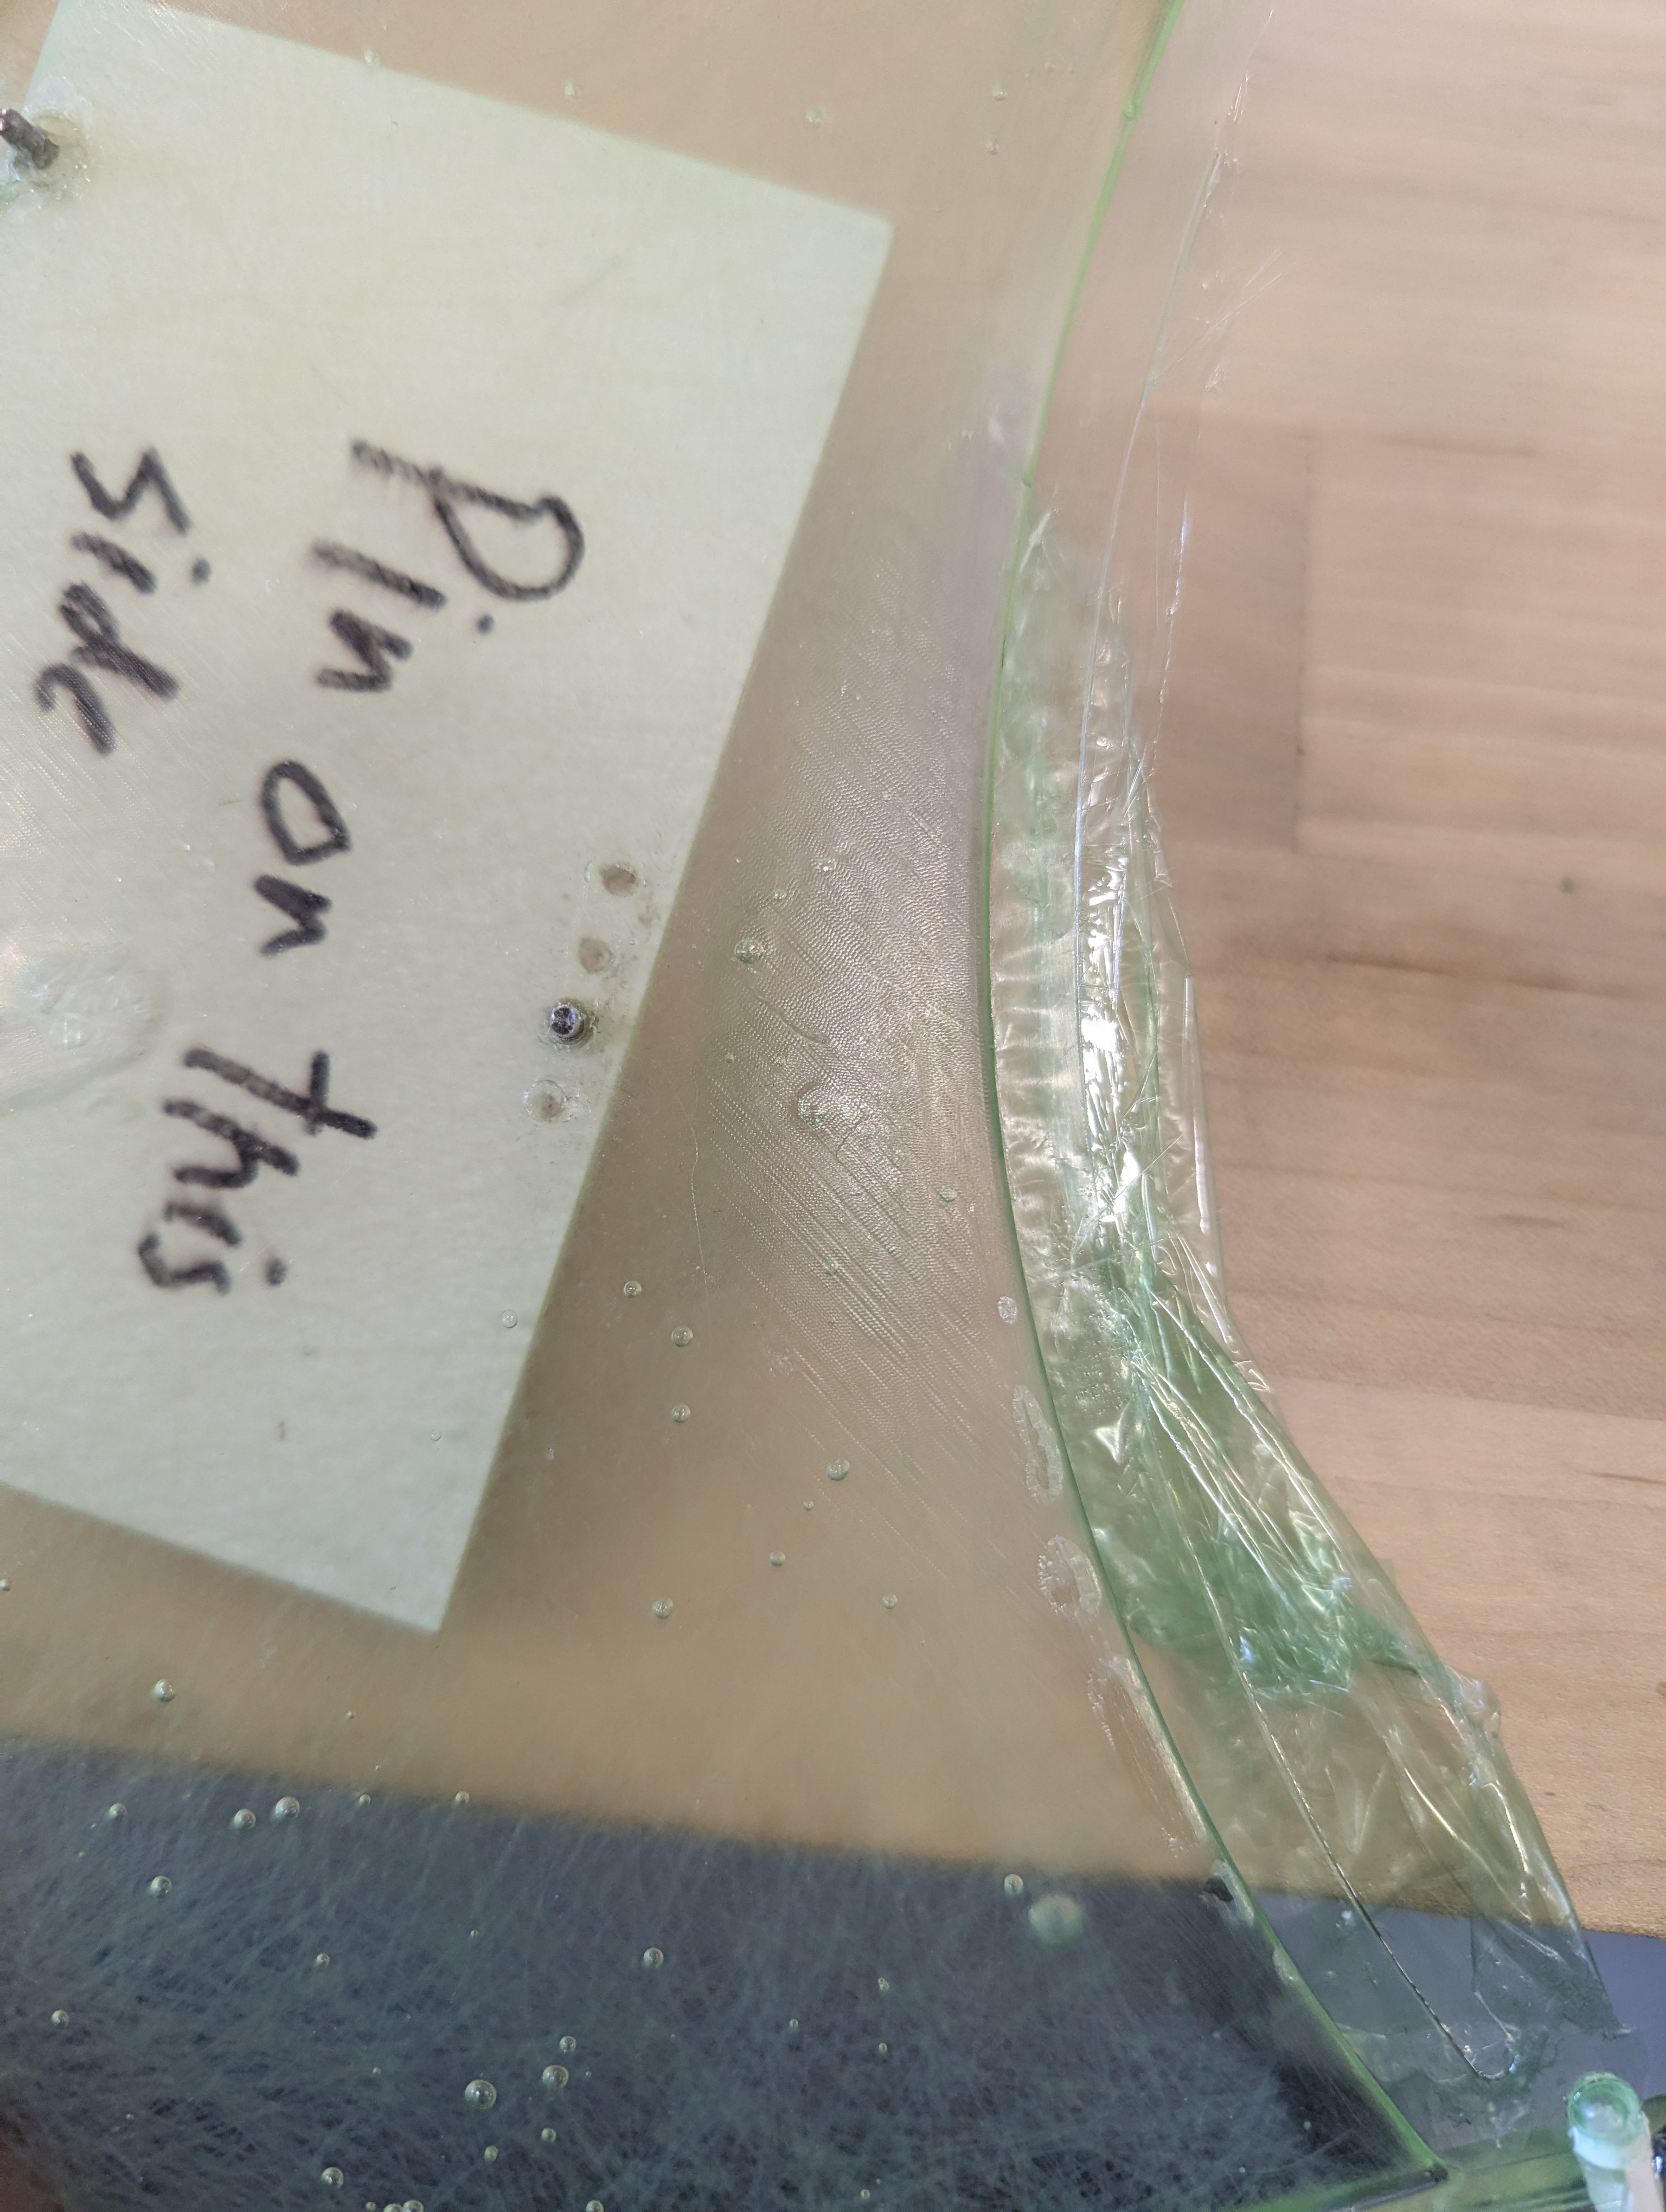
\includegraphics[height=0.5\textheight,keepaspectratio]{images/sf_charge_pin_bubbles_2.jpg}
    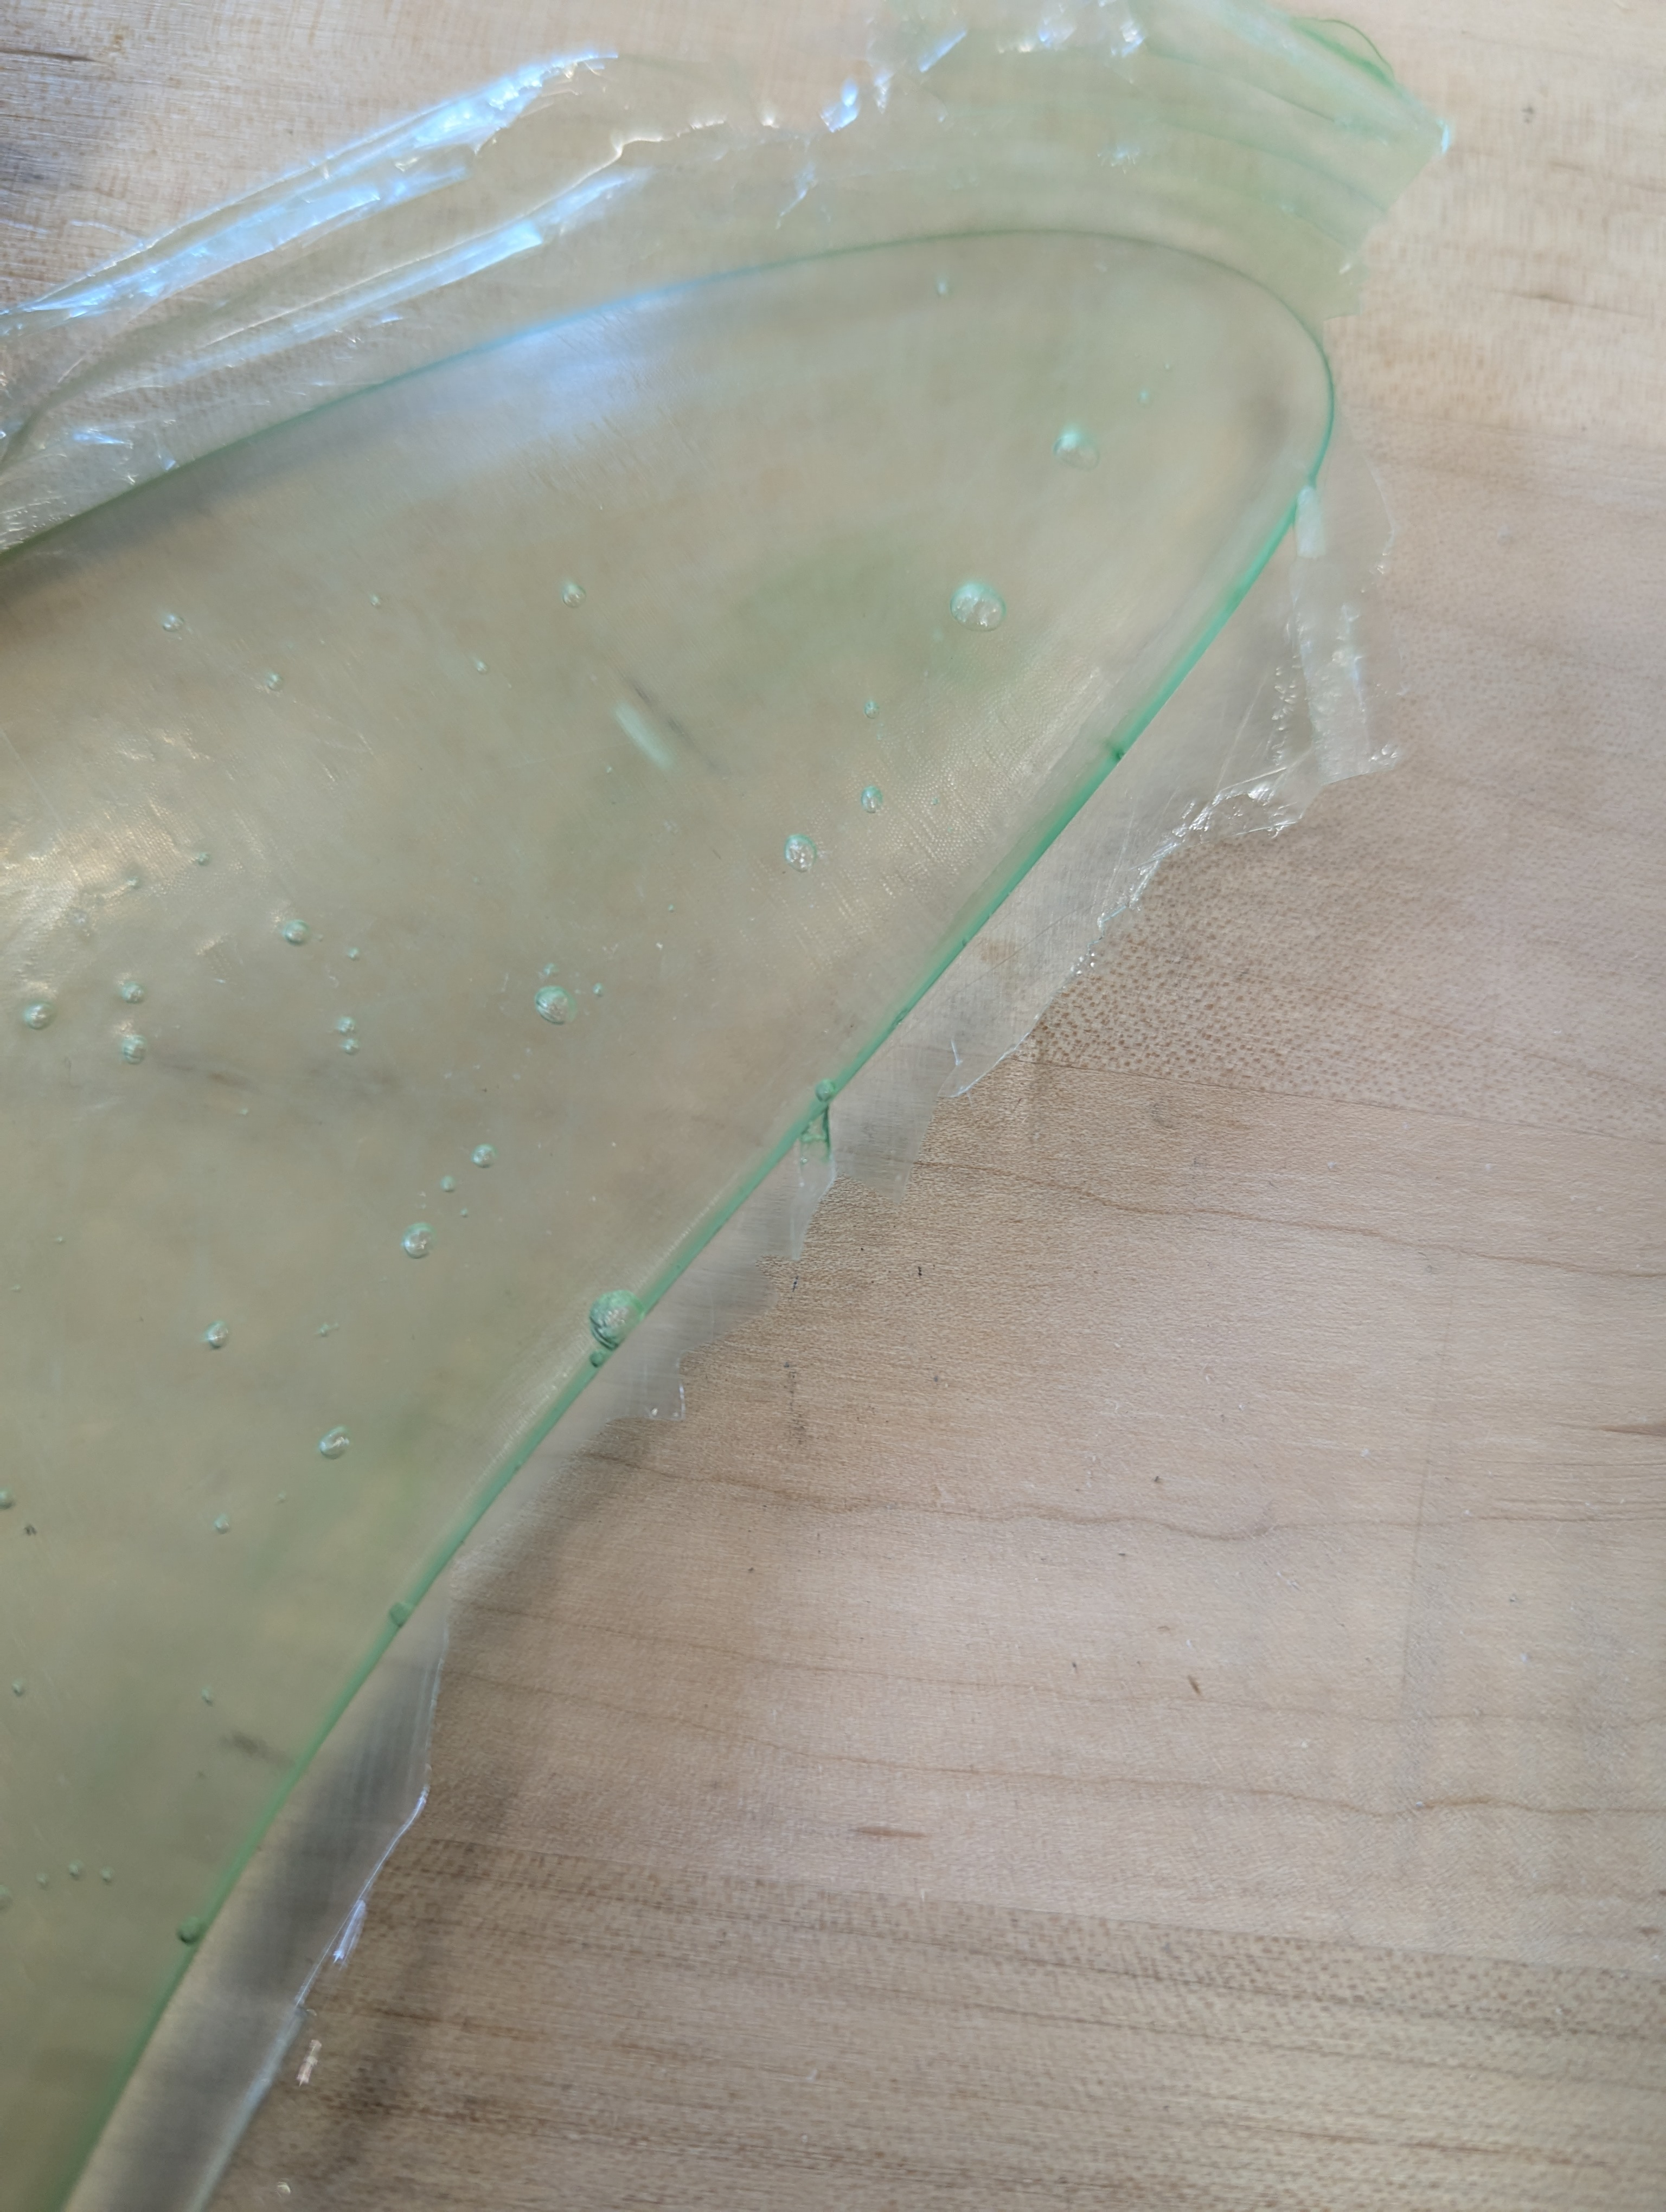
\includegraphics[height=0.5\textheight,keepaspectratio]{images/sf_tip_bubbles.jpg}
    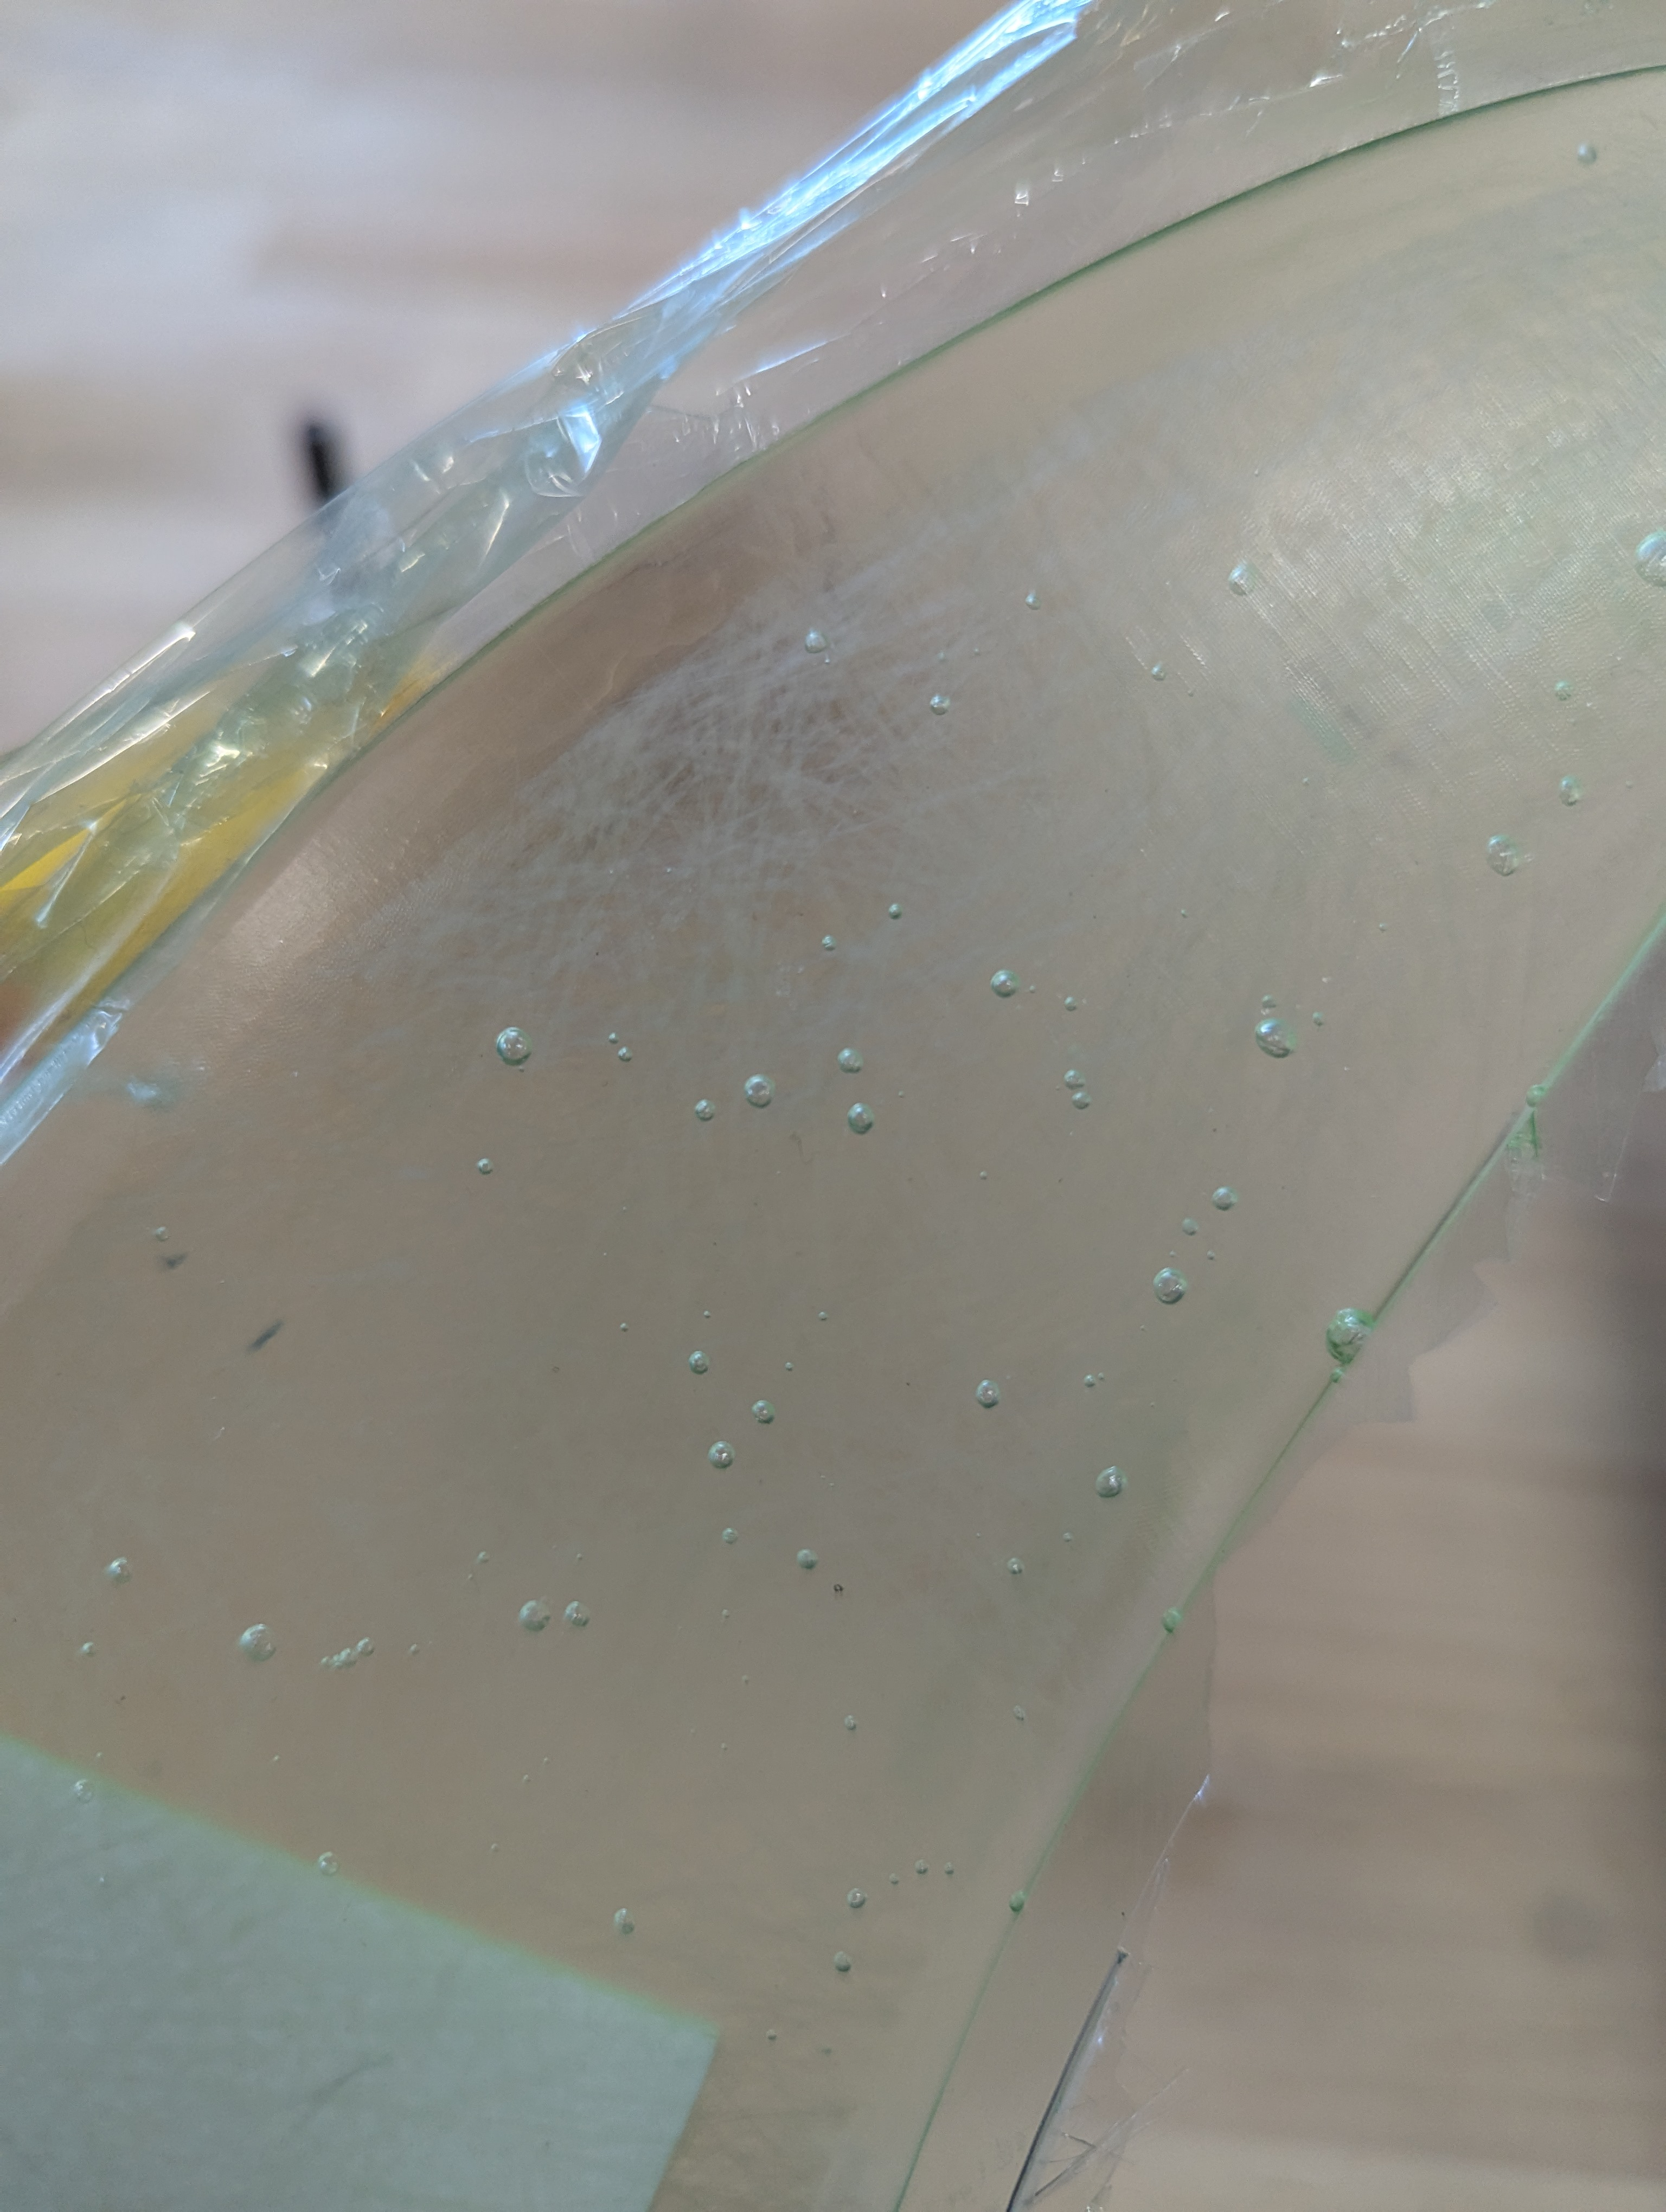
\includegraphics[height=0.5\textheight,keepaspectratio]{images/sf_tip_bubbles_2.jpg}
    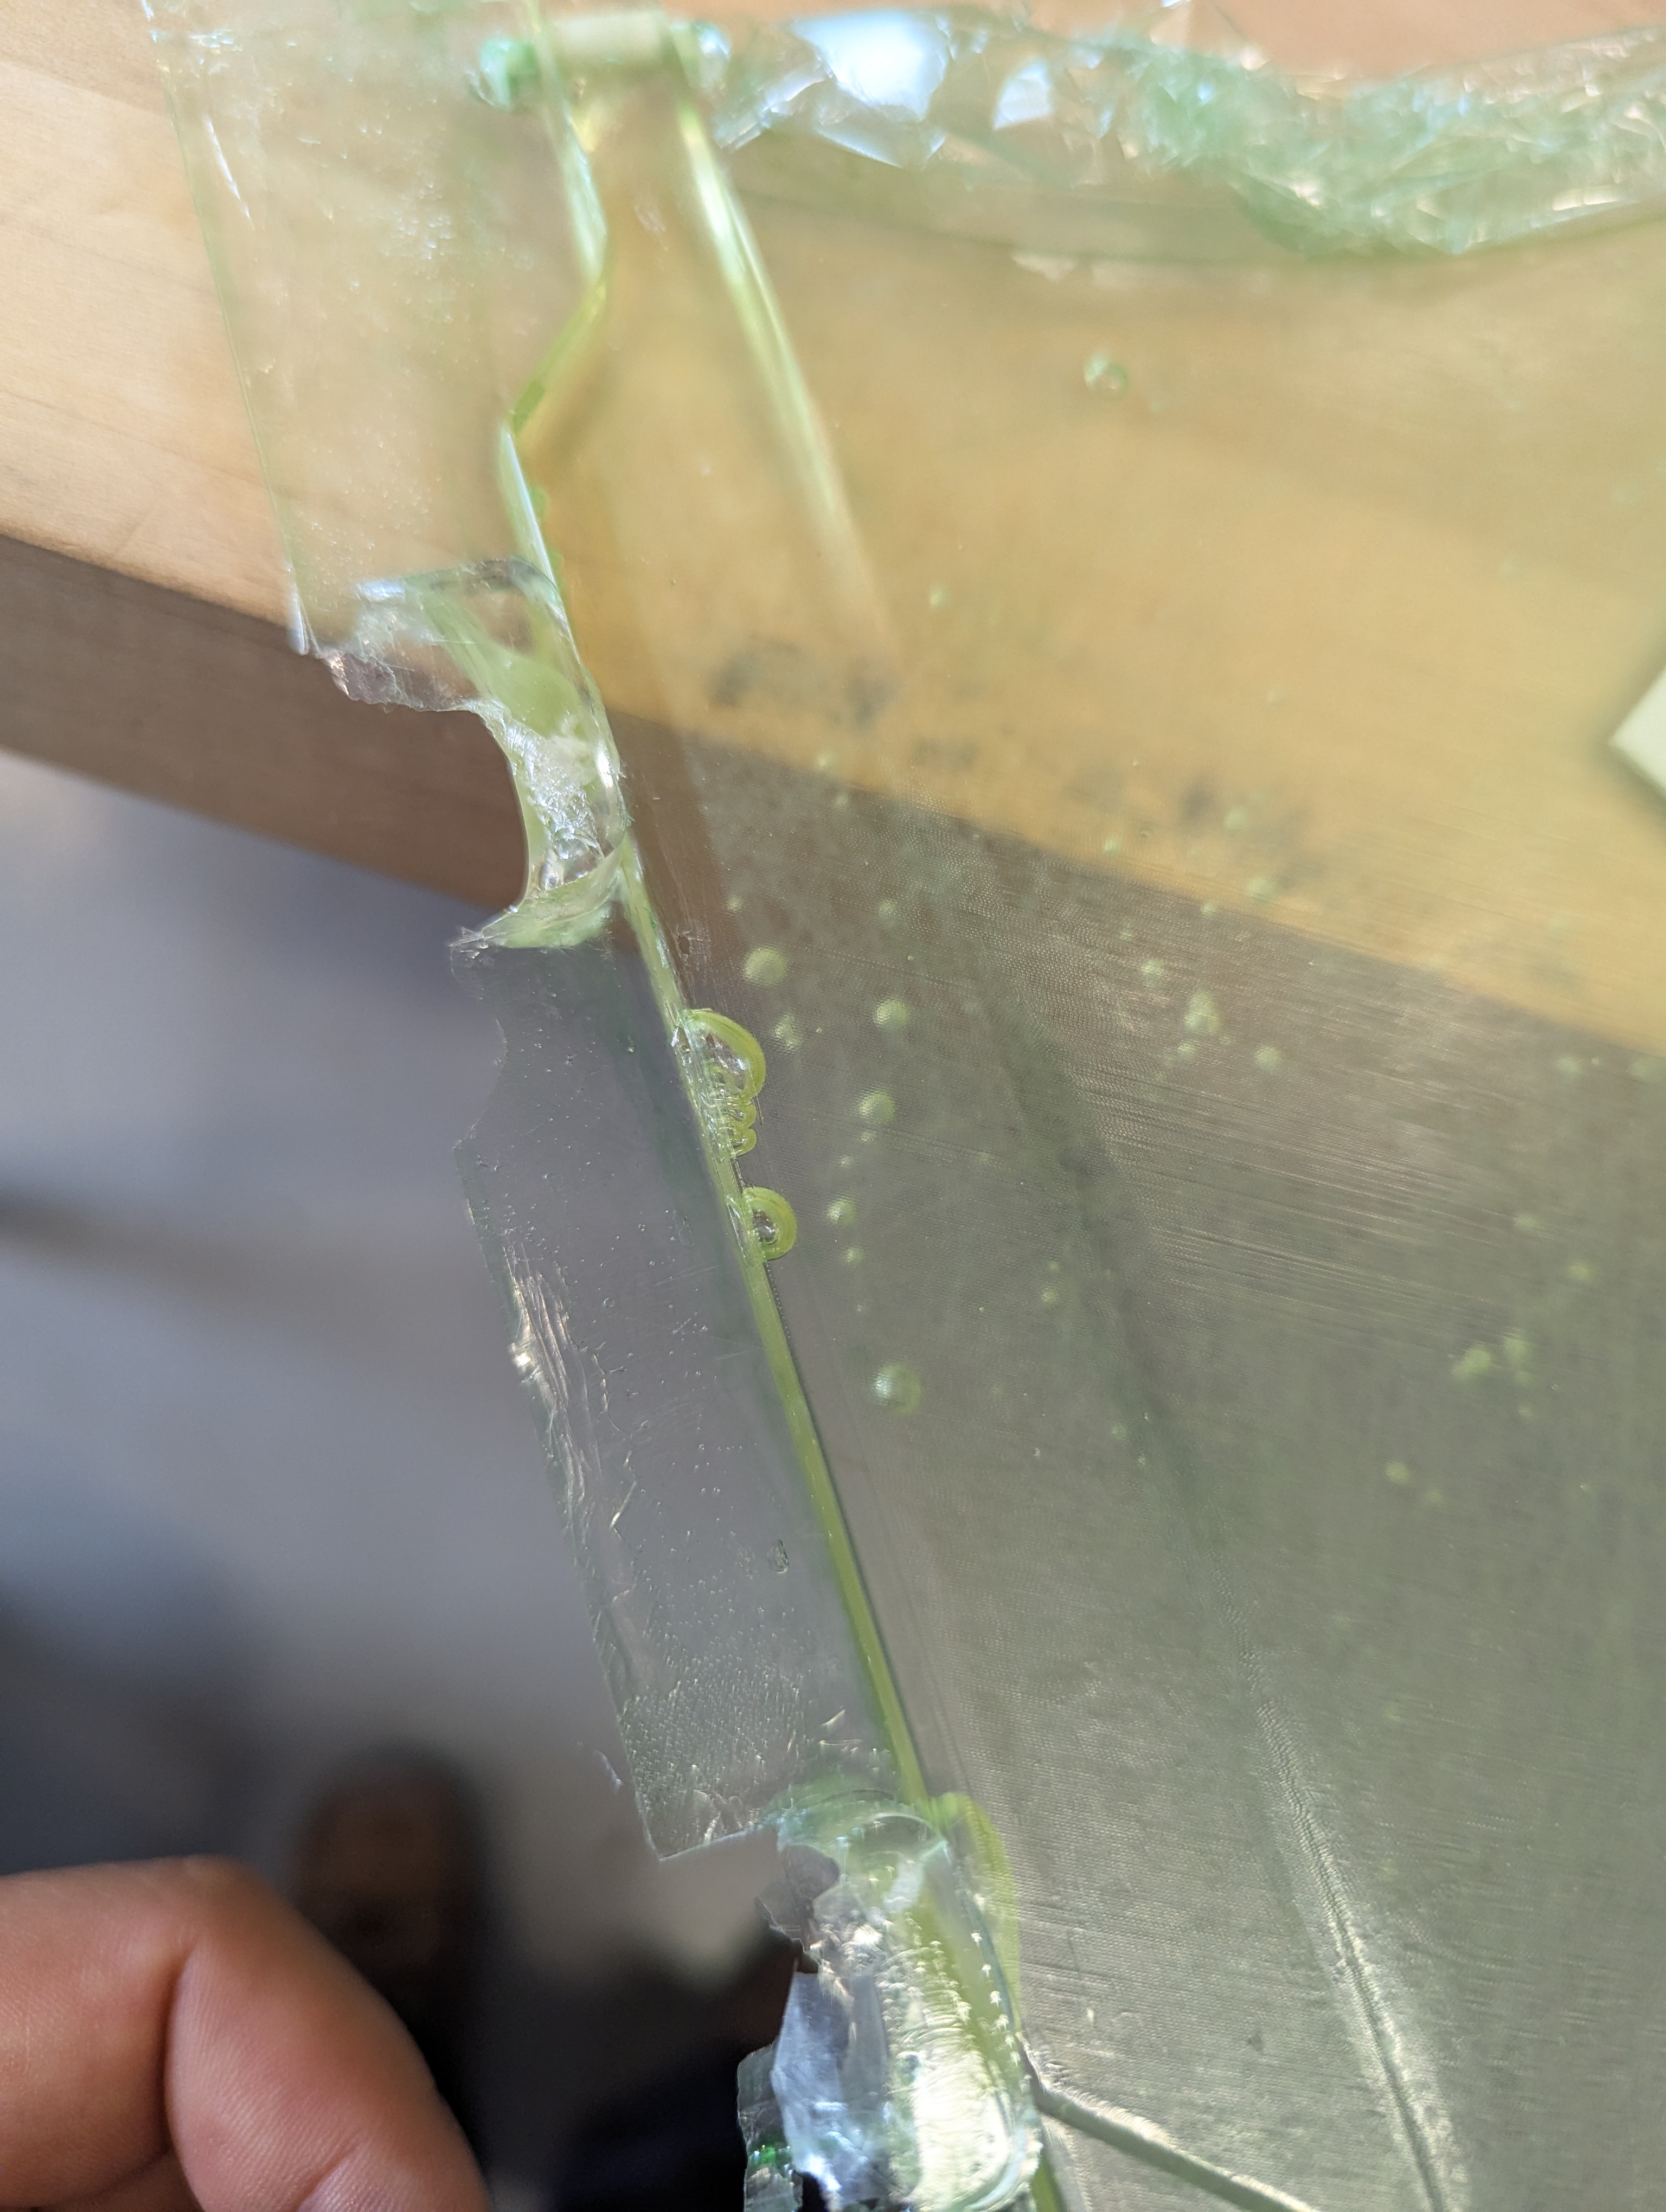
\includegraphics[height=0.5\textheight,keepaspectratio]{images/sf_root_bubbles_3.jpg}
\end{frame}

\begin{frame}{Breaks}
    \centering
    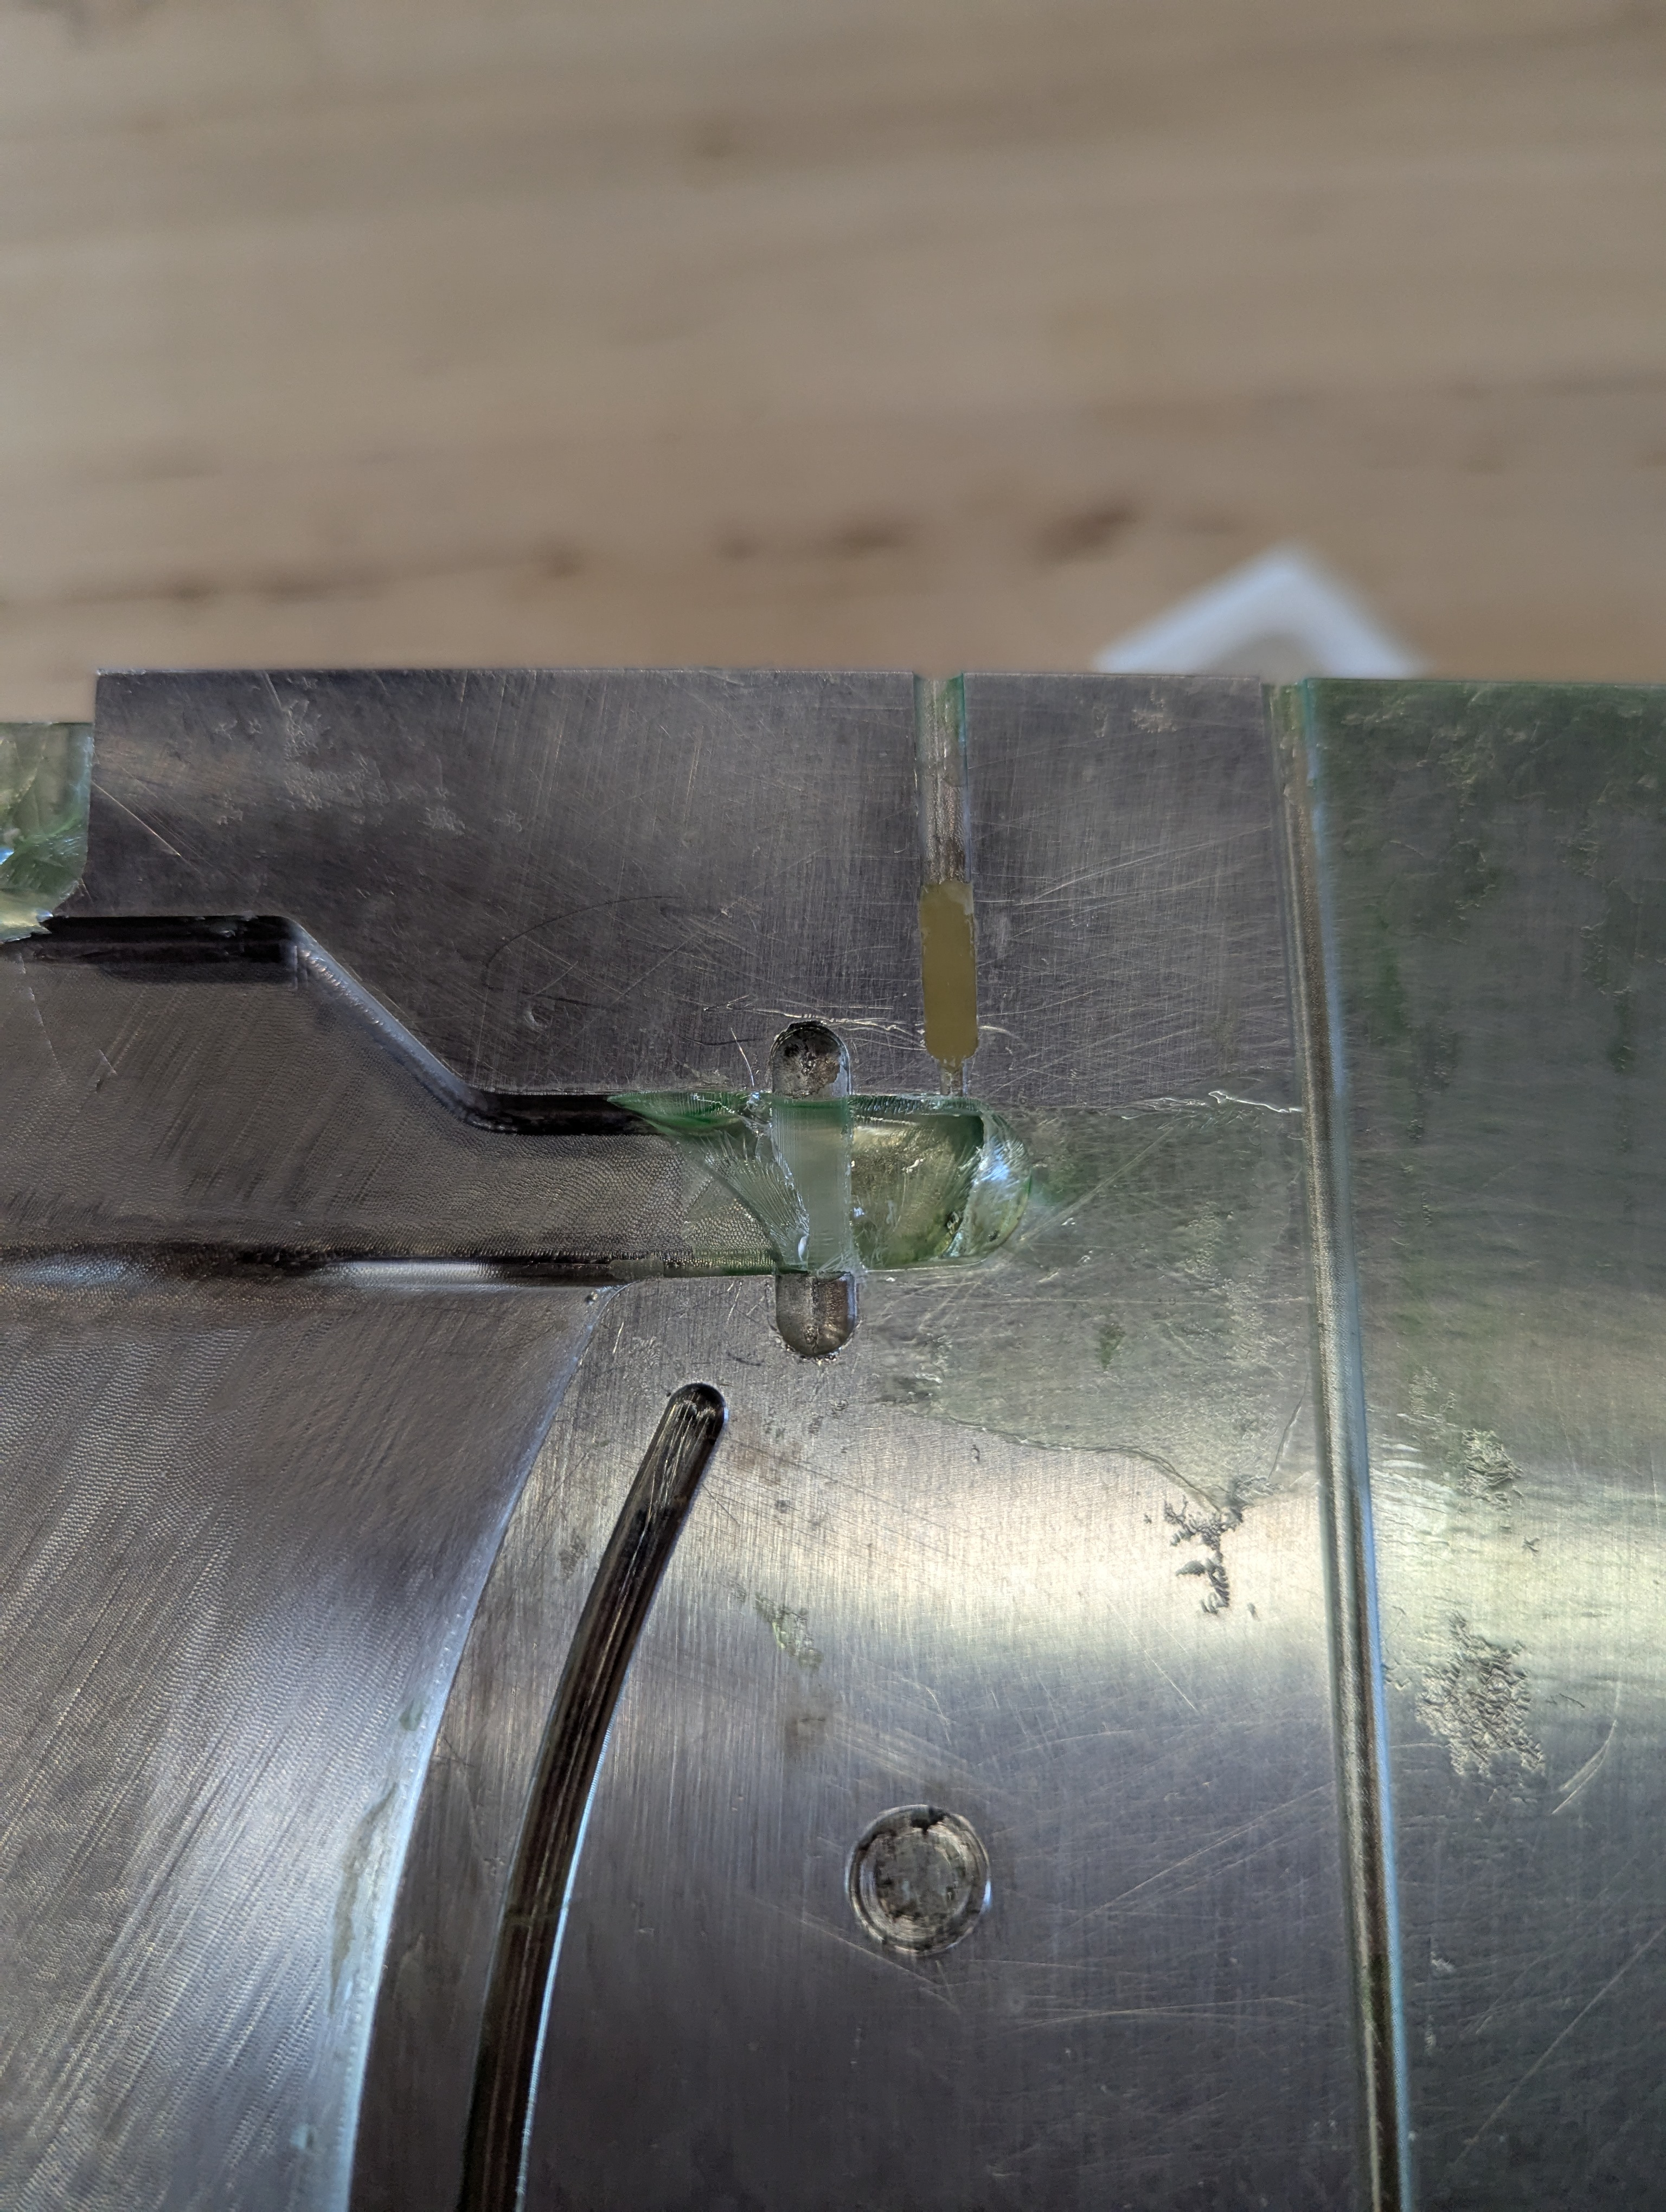
\includegraphics[height=0.5\textheight,keepaspectratio]{images/sf_mold_tail_broken.jpg}
    
\includegraphics[height=0.5\textheight,keepaspectratio]{images/sf_tail_broken.jpg}
    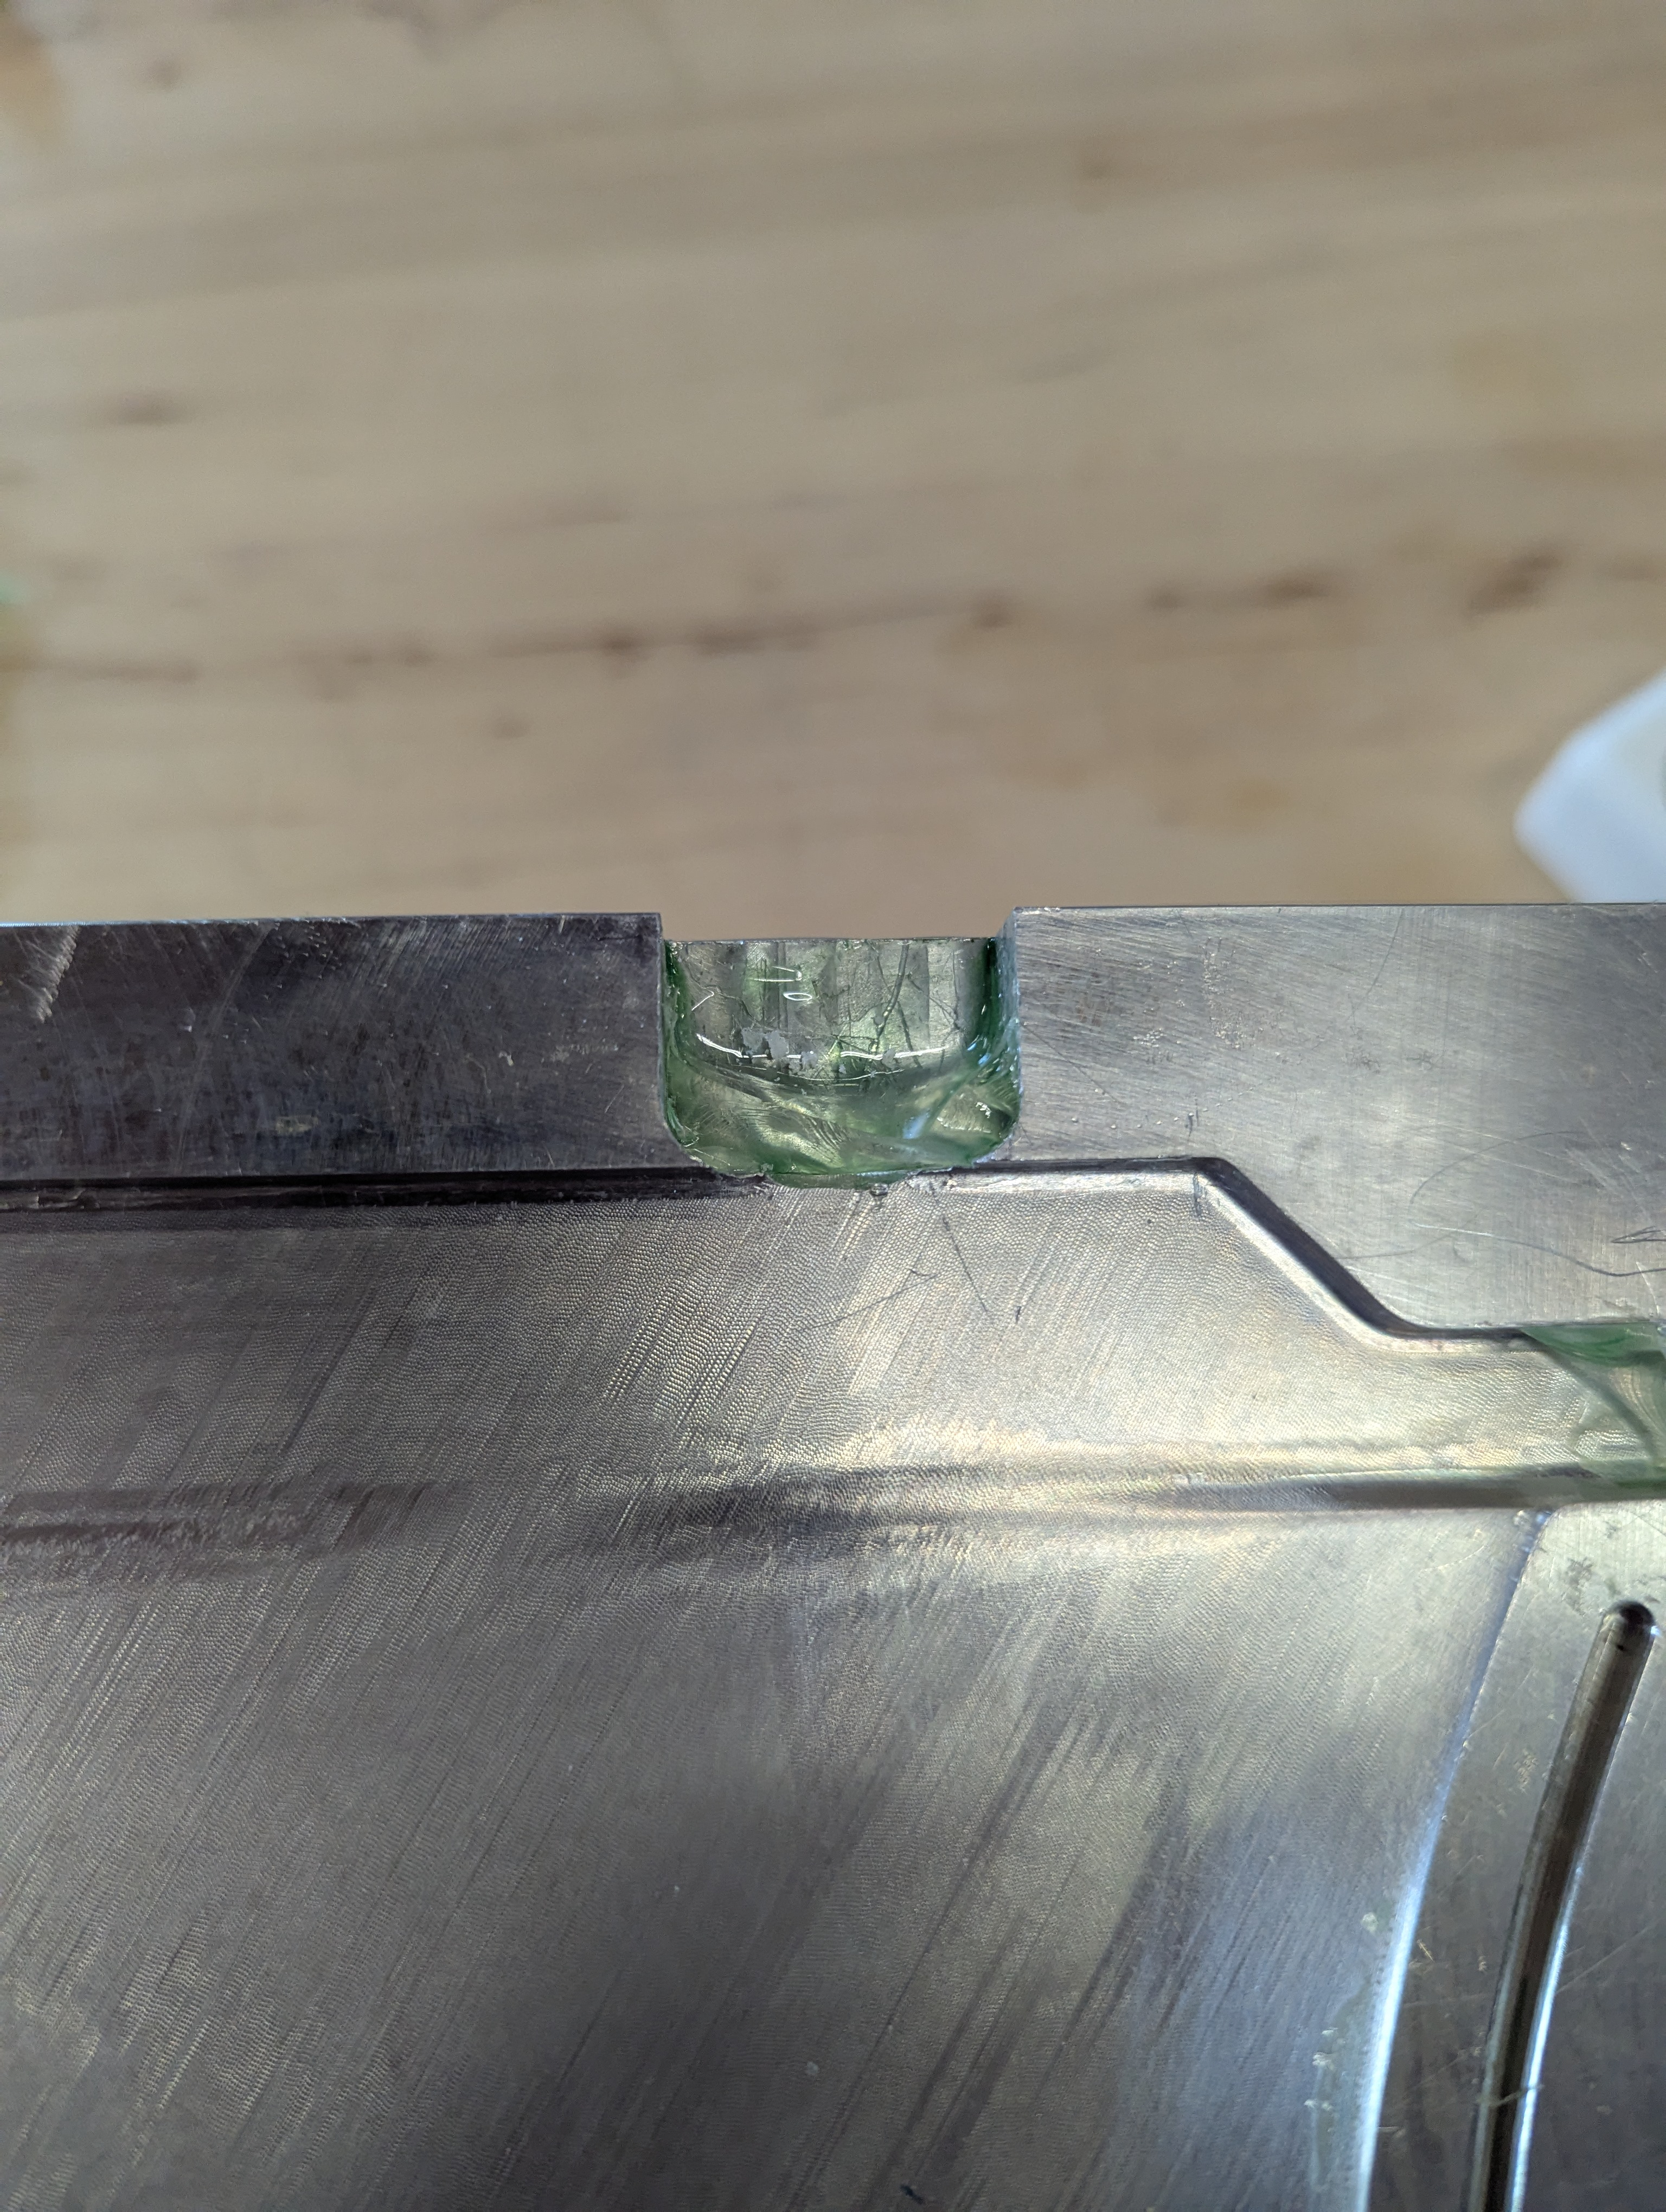
\includegraphics[height=0.5\textheight,keepaspectratio]{images/sf_mold_tailpour_broken.jpg}
    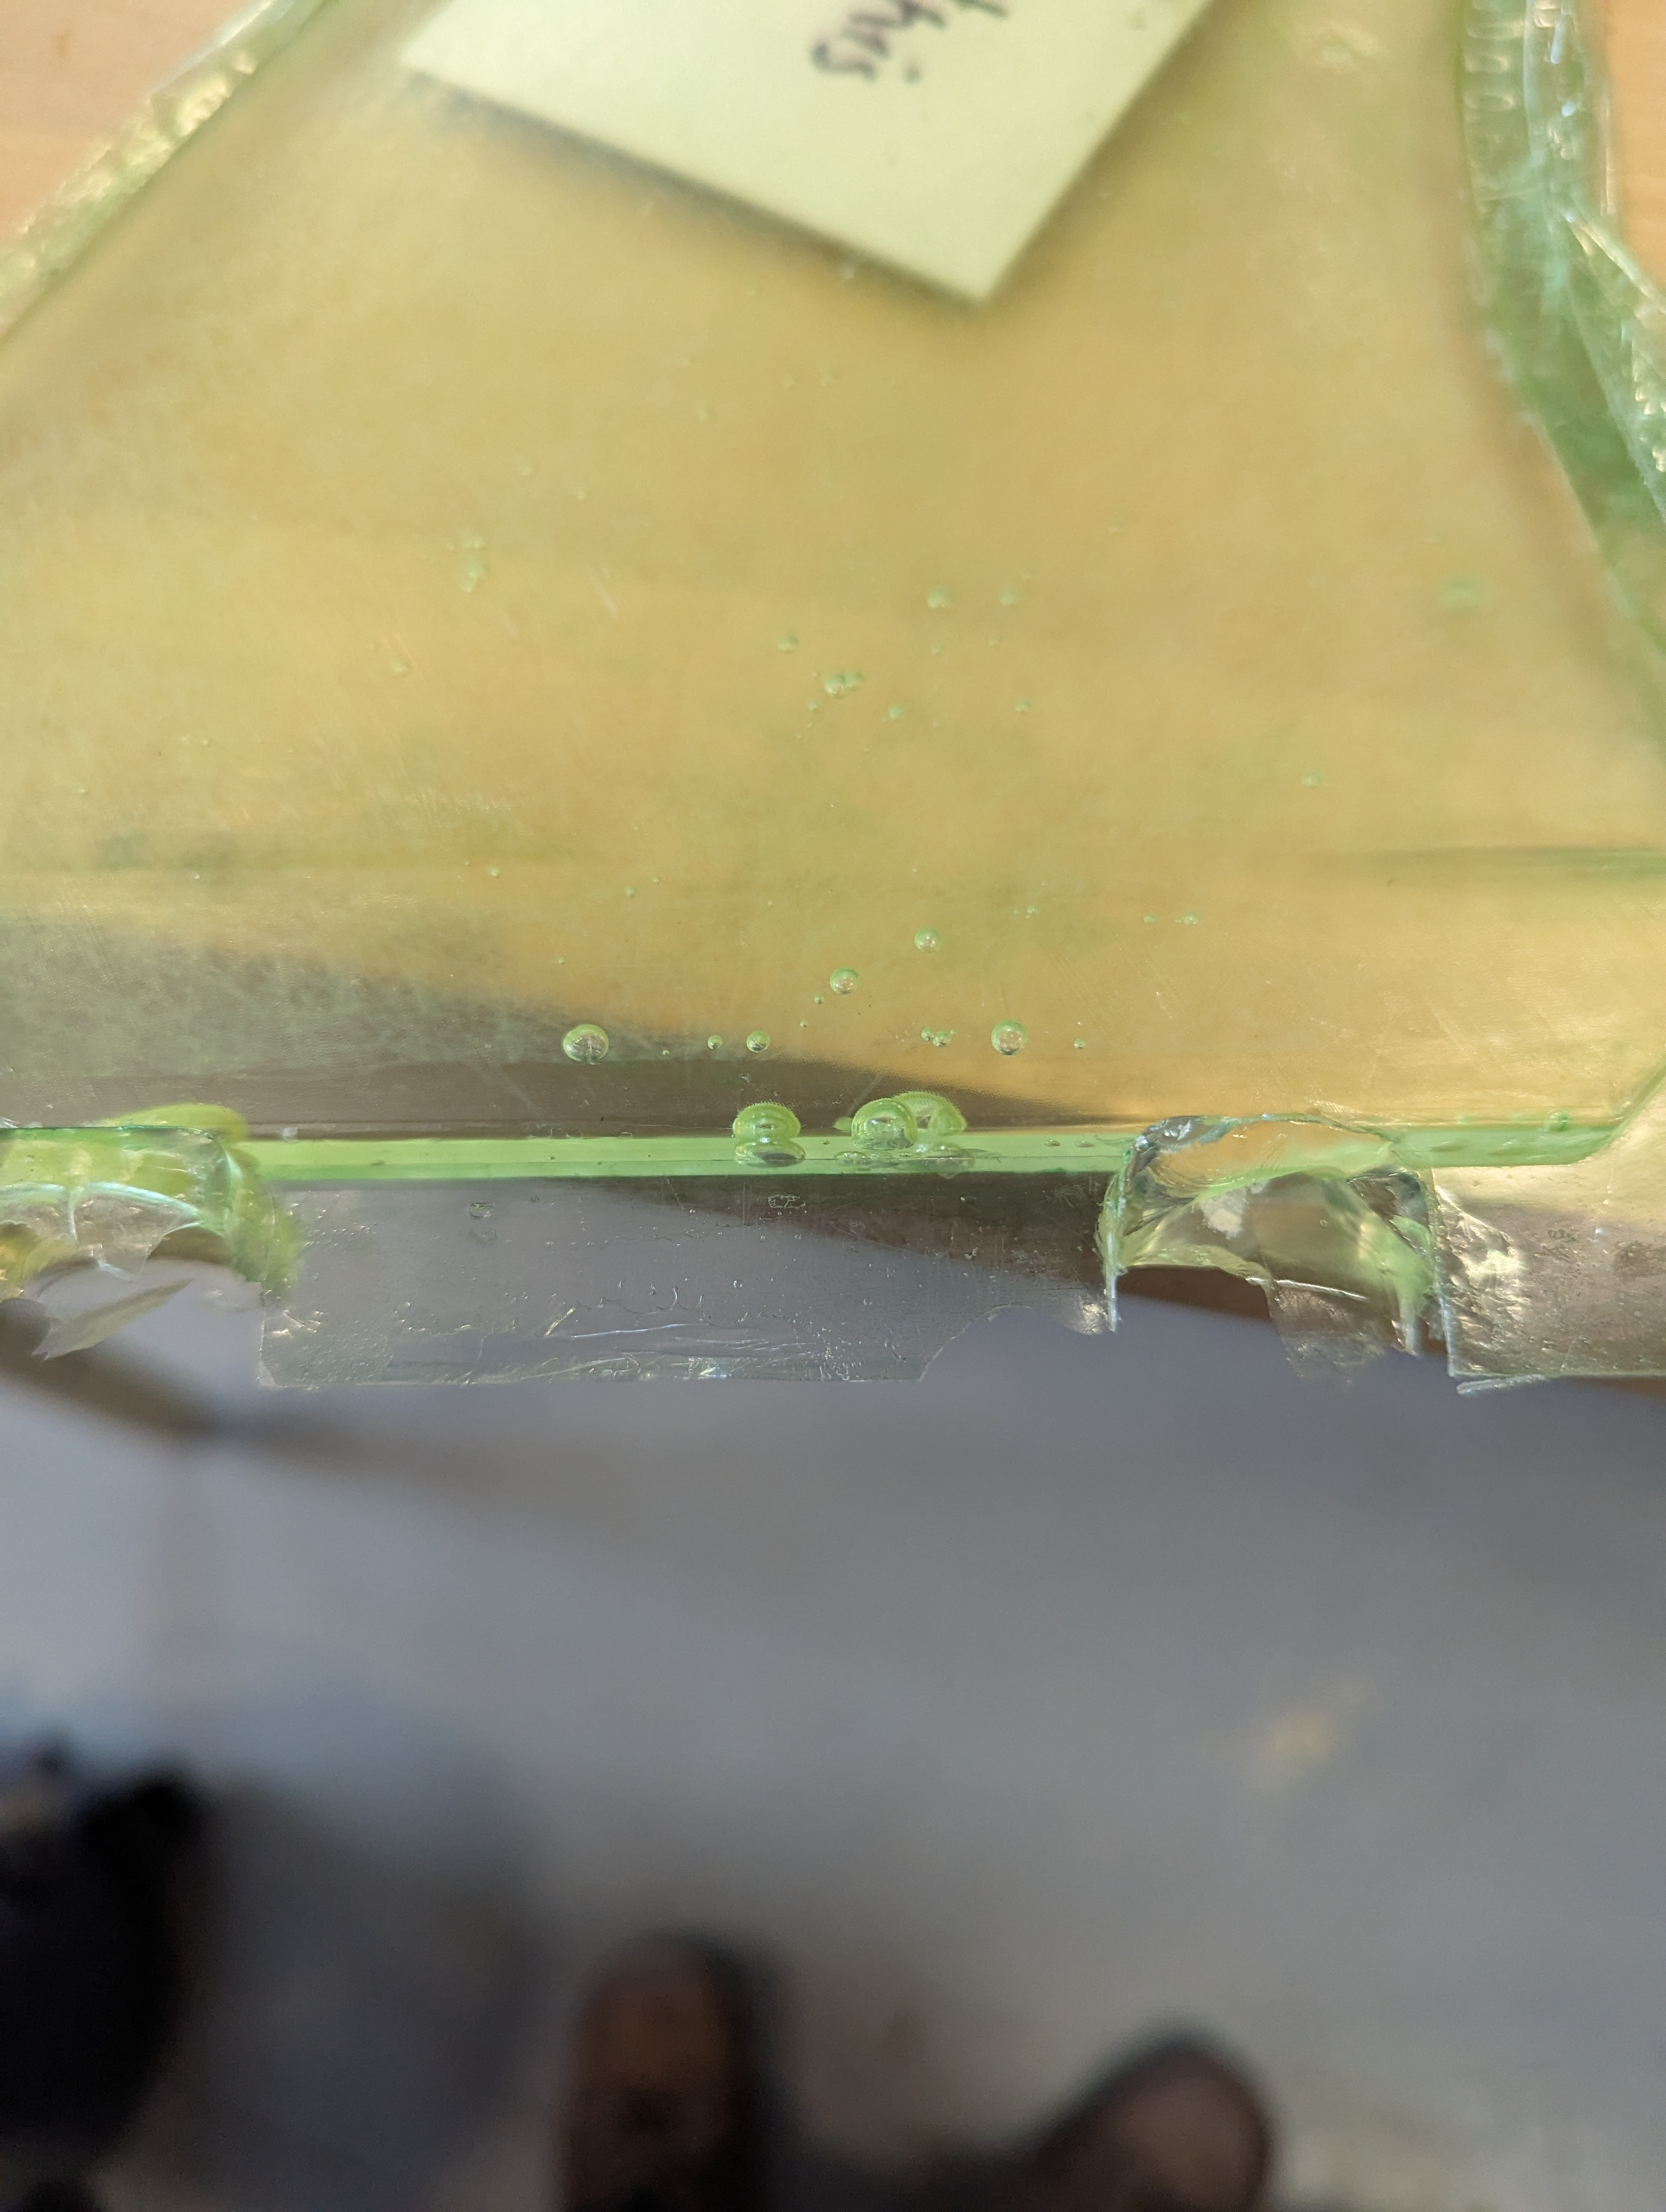
\includegraphics[height=0.5\textheight,keepaspectratio]{images/sf_root_bubbles.jpg}
\end{frame}

\begin{frame}{Resin Leakage}
    \centering
    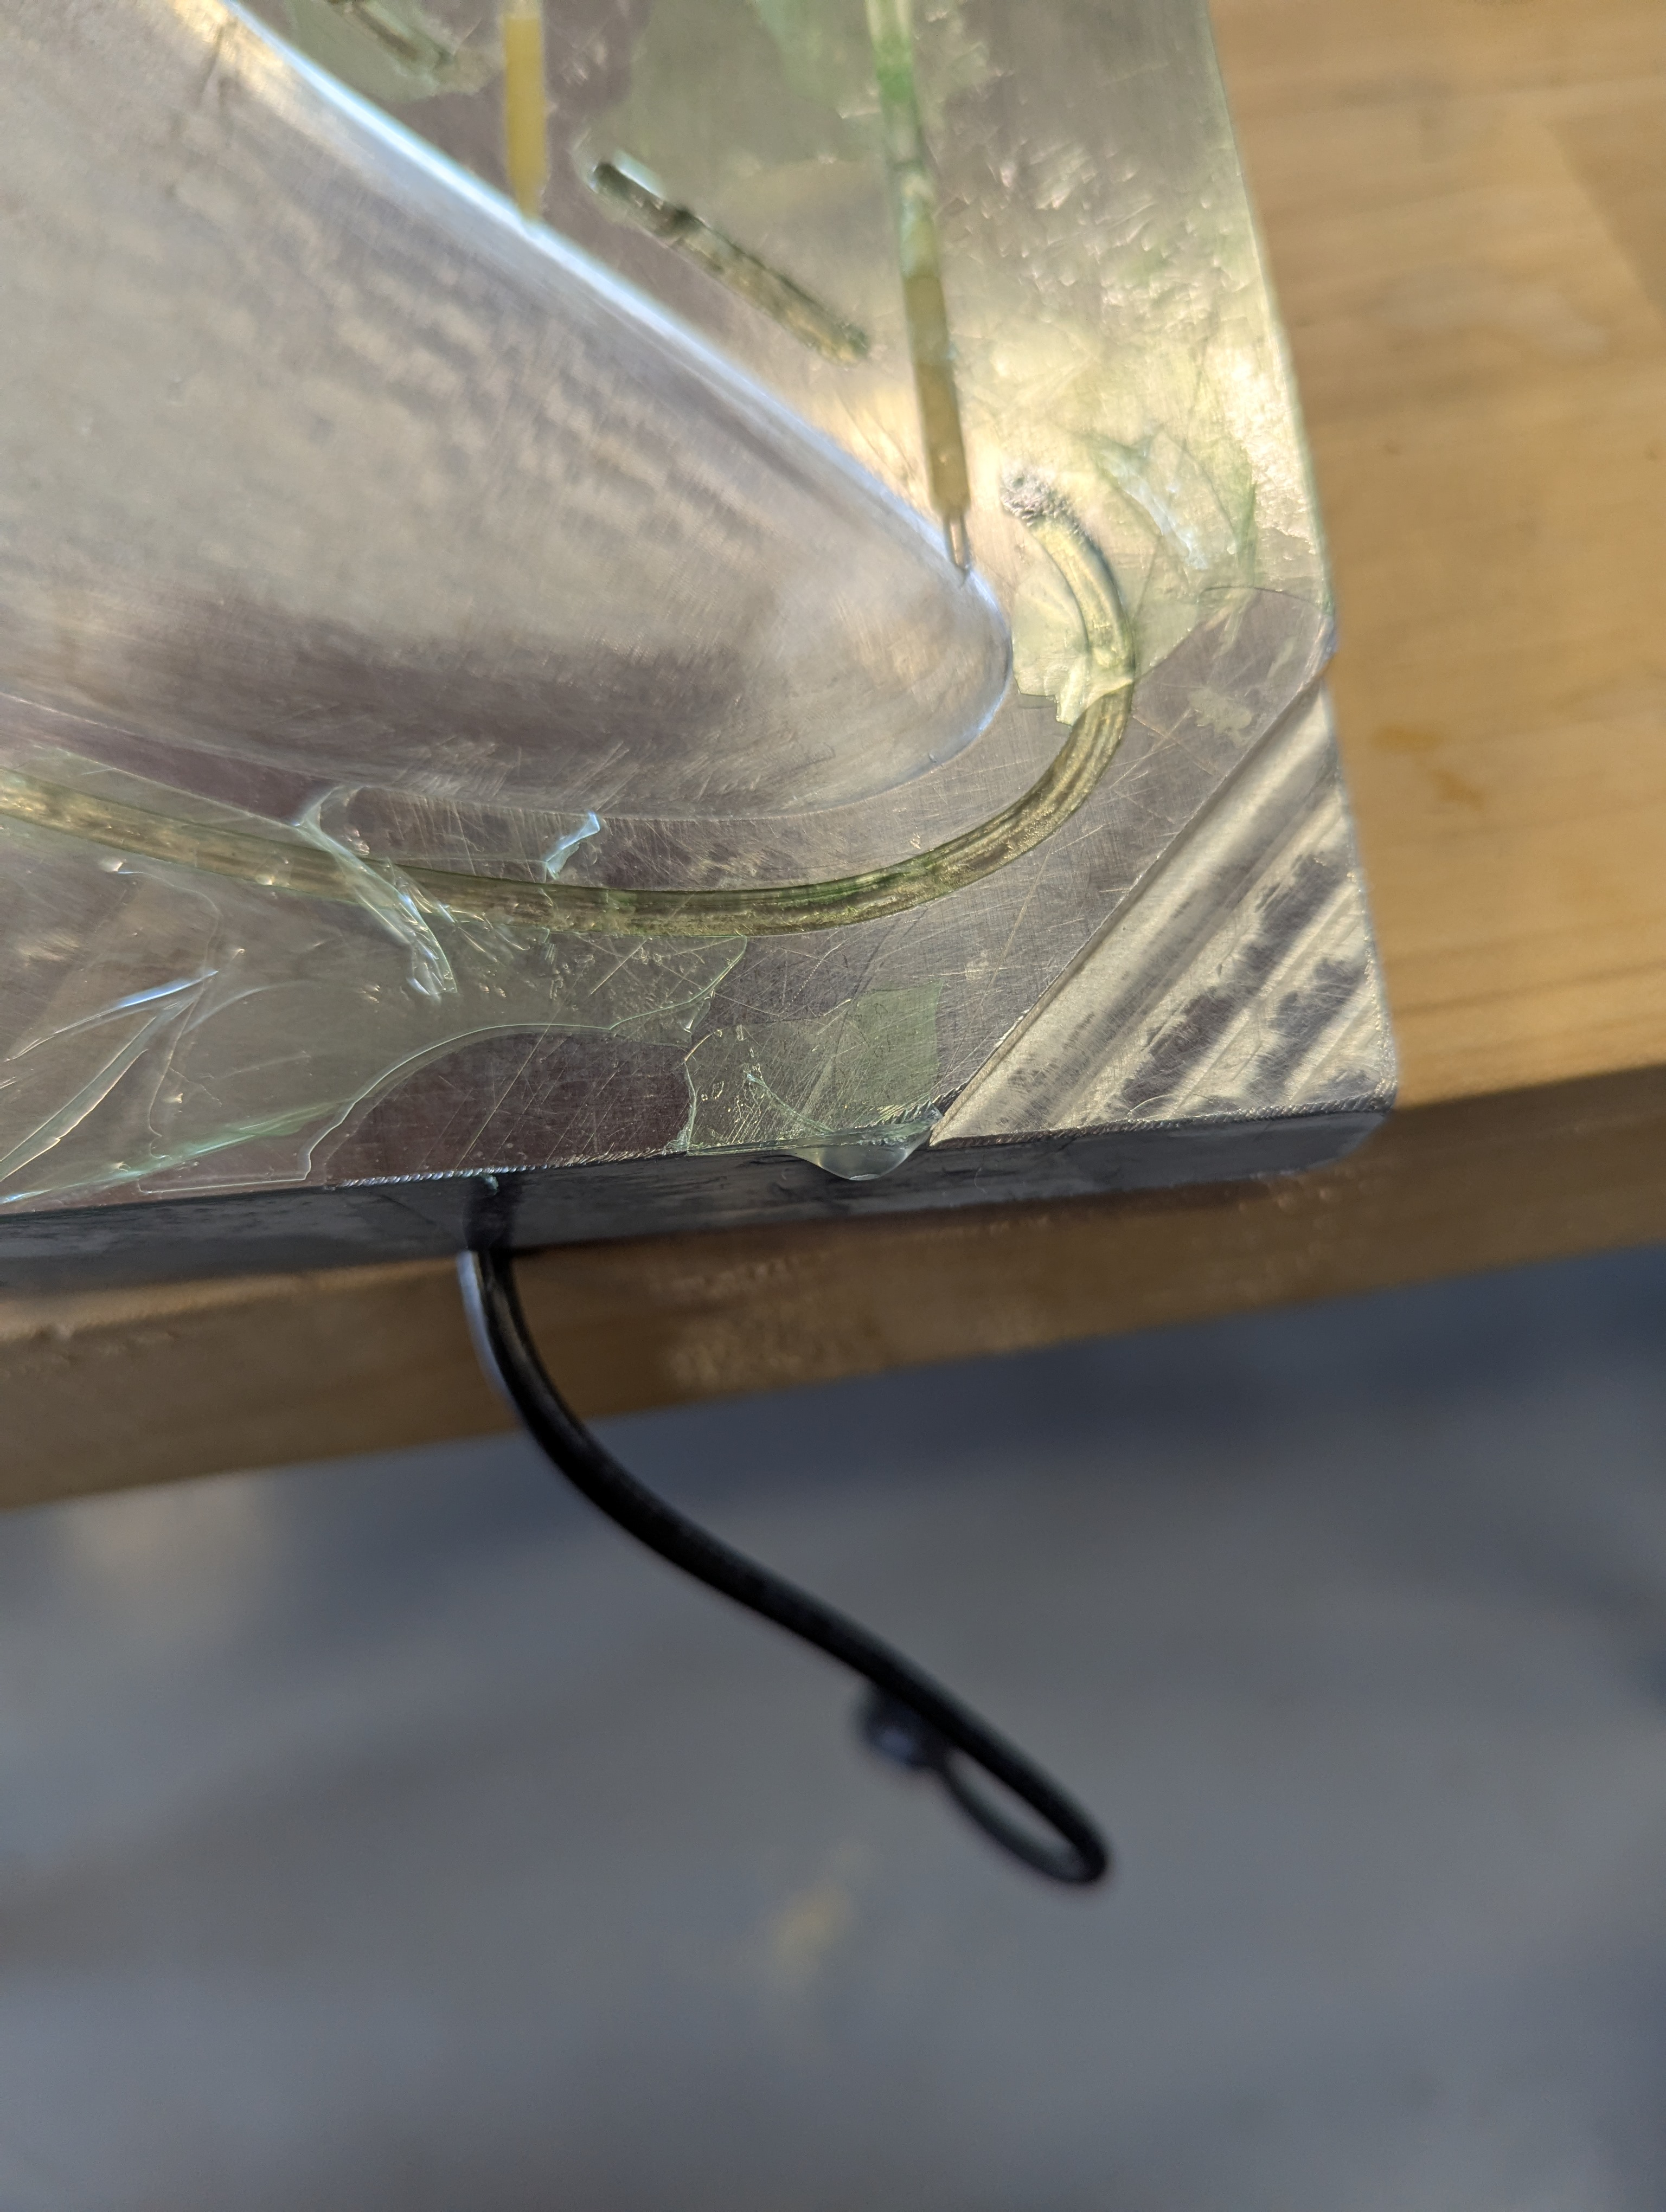
\includegraphics[height=0.5\textheight,keepaspectratio]{images/sf_mold_tip_leakage.jpg}
    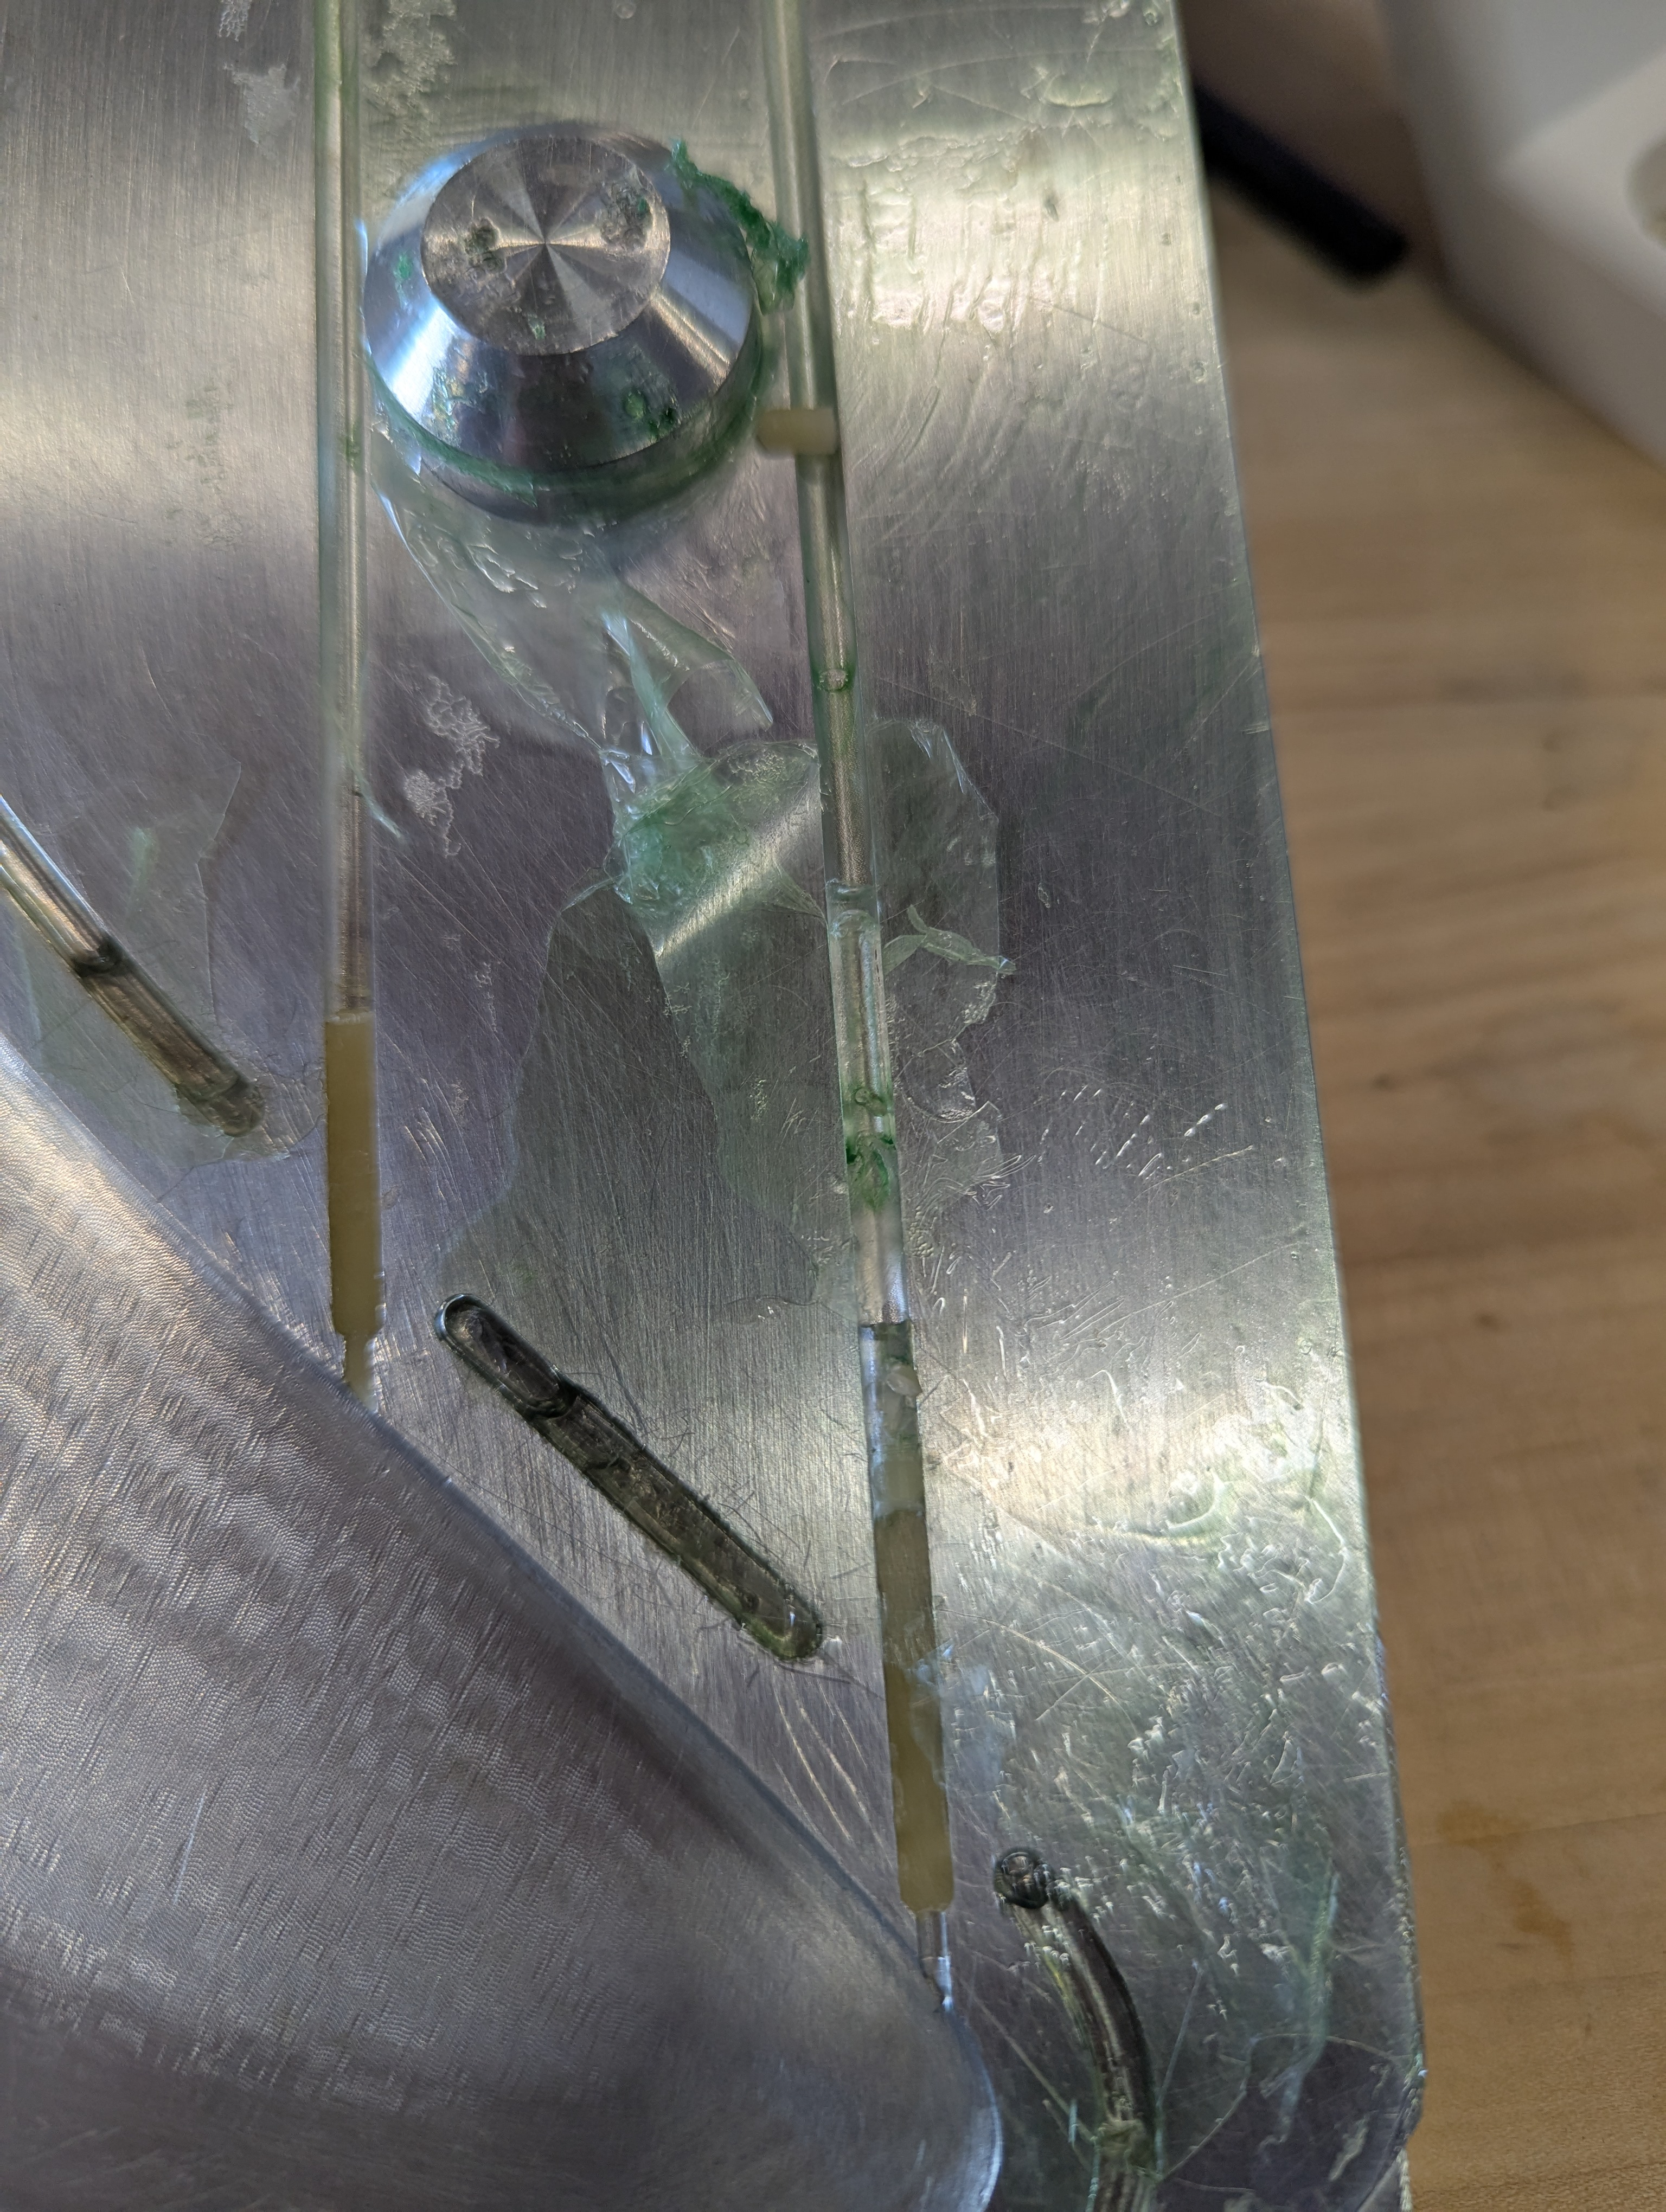
\includegraphics[height=0.5\textheight,keepaspectratio]{images/sf_mold_tipAirTube_flooded.jpg}
    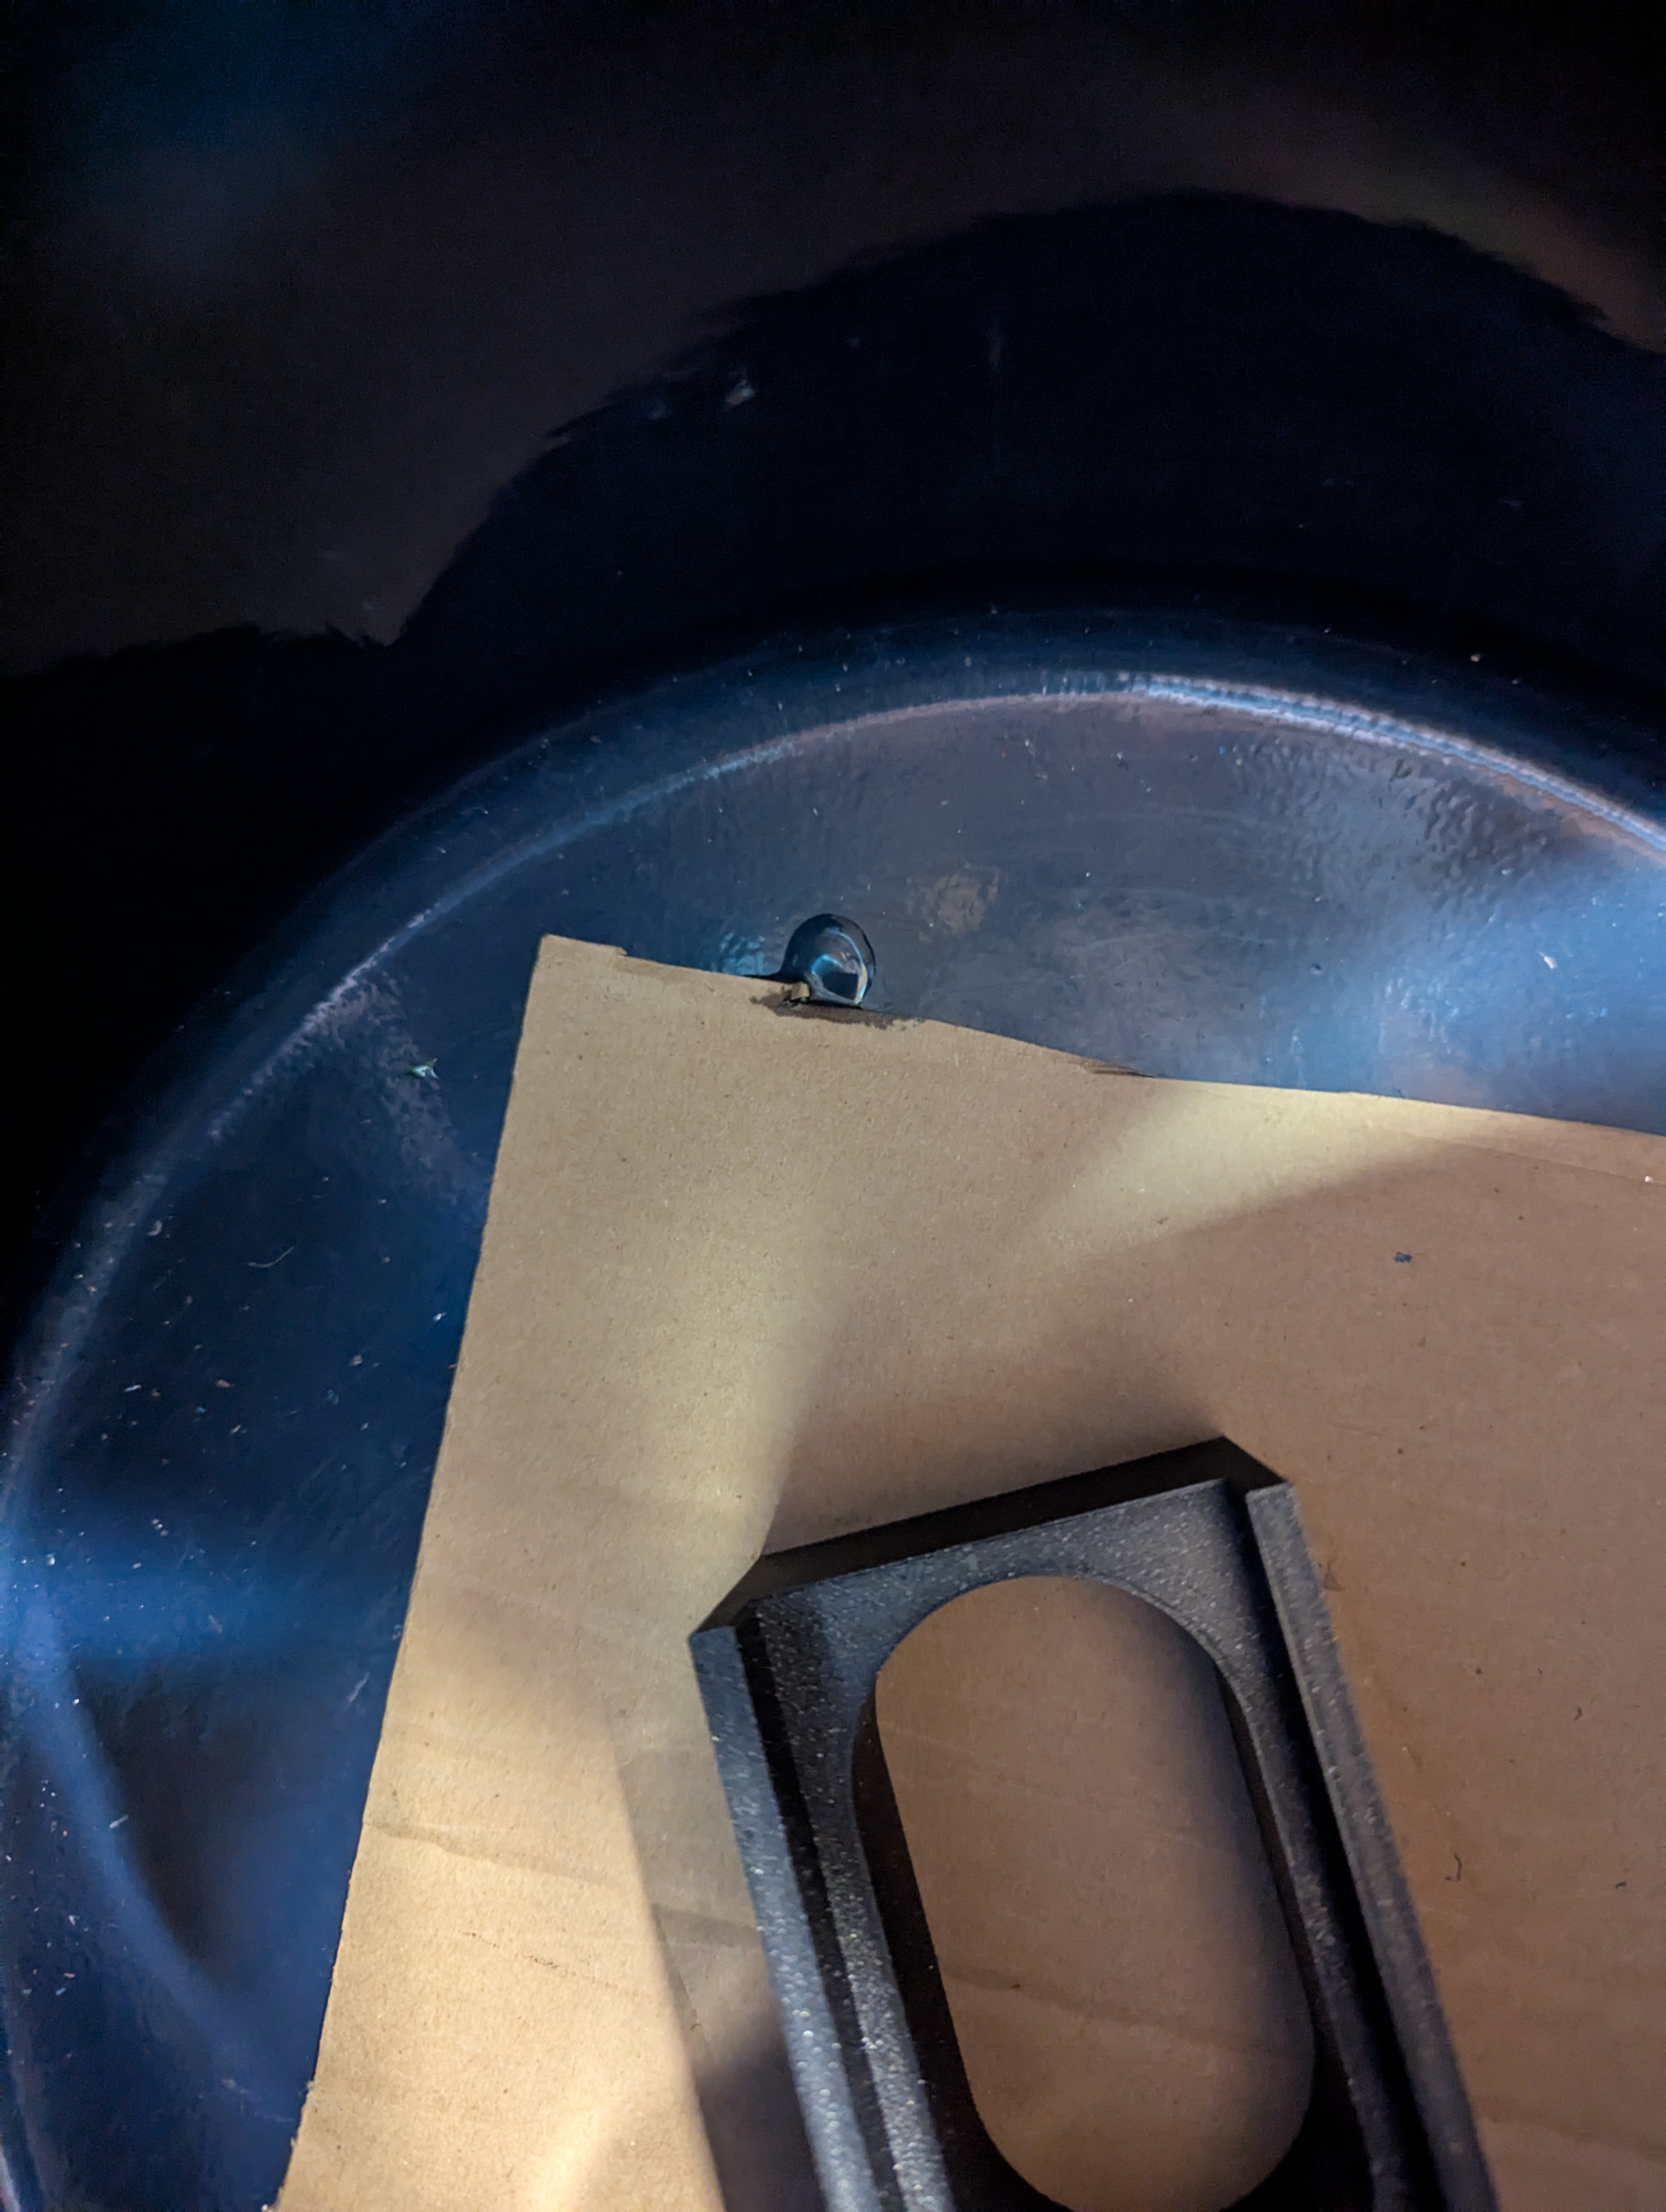
\includegraphics[height=0.5\textheight,keepaspectratio]{images/sf_pot_leakage.jpg}
\end{frame}

\begin{frame}{Firmware}
    \begin{itemize}
        \item DMP Driver
        \item Threading
        \item Data Endpoint - WIP
    \end{itemize}
\end{frame}

% To create a slide with a bullet list, use the following:
% \begin{frame}{TITLE}
%     \begin{itemize}
%         \item ITEM 1
%         \item ITEM 2
%     \end{itemize}    
% \end{frame}

% To create a slide with numbered list, use the following:
% \begin{frame}{TITLE}
%     \begin{enumerate}
%         \item ITEM 1
%         \item ITEM 2
%     \end{enumerate}
% \end{frame}

% To create a slide with a graphic:
% 1. Add the graphic to this folder (named picture.png)
% 2. Use the following:
% \begin{frame}{TITLE}
%     \centering
%     \includegraphics[height=0.7\textheight,width=0.7\textwidth,keepaspectratio]{picture.png}
% \end{frame}

% To create a slide with two columns, use the following:
% \begin{frame}{TITLE}
%     \begin{columns}
%         \begin{column}{0.5\textwidth}
%             COLUMN 1 BODY
%         \end{column}
%         \begin{column}{0.5\textwidth}
%             COLUMN 2 BODY
%         \end{column}
%     \end{columns}
% \end{frame}
